\RequirePackage{silence}
\WarningFilter{biblatex}{Patching footnotes failed}
\documentclass[10pt, compress,british,xcolor={svgnames,dvipsnames,x11names},trans]{beamer}

\usepackage{babel}
\usepackage{csquotes}
\usepackage{comment}
\usepackage{tikzsymbols}
% Wenyin used these packages
\usepackage{marginnote}
\usepackage{longtable}
\usepackage{url}
\usepackage{hyperref}
\usepackage{wasysym} % for checkboxes
\usepackage{mathtools} % for overbrace and underbrace
\usepackage{enumerate} % for style setting in itemize
%%% mtheme customisations
\usetheme[progressbar=frametitle,block=fill]{m}
\setmonofont[Scale=0.92]{Fira Mono}
\AtBeginSubsection{
\metroset{color/background=dark}
\frame[plain,c]{
  \begin{center}
  \begin{minipage}{25em}
    \usebeamercolor[fg]{section title}
    \usebeamerfont{section title}
    \insertsubsection\\[-1ex]
    \usebeamertemplate*{progress bar in section page}
  \end{minipage}
  \end{center}
}
\metroset{color/background=light}
}
%%%%% end mtheme

\setbeamertemplate{frametitle continuation}[from second]
\setbeamertemplate{bibliography item}[book]

\usepackage{xeCJK}
\setCJKmainfont{cwTeXFangSong}
% \setCJKsansfont[BoldFont=Kozuka Gothic Pro]{Kozuka Gothic Pro L}
\setCJKsansfont{IPAGothic}
% \newCJKfontfamily{\xiheifont}[BoldFont=STHeiti]{STXihei}
\newCJKfontfamily{\xiheifont}{WenQuanYi Micro Hei}

\usetikzlibrary{arrows}
\usetikzlibrary{chains}
\usepackage{tikz-qtree}
\usepackage{multicol}


\usepackage{expex}
%\lingset{glhangindent=2em,glspace=1em,aboveexskip=0pt,belowexskip=0pt,aboveglftskip=-3pt,extraglskip=3pt} %v0.1
%\lingset{exskip=0pt,interpartskip=-3pt,belowpreambleskip=-3pt,belowglpreambleskip=-3pt,aboveglftskip=-3pt,extraglskip=3pt,glhangstyle=none}
\usepackage{relsize}
\usepackage{booktabs,tabularx}
%\usepackage{textcomp}
\usepackage{listings}
\lstset{basicstyle=\ttfamily,breaklines=true,breakatwhitespace=true,
keywordstyle={\color{NavyBlue}\bfseries}, showstringspaces=false,
commentstyle={\color{PaleVioletRed4}},
emphstyle={\color{OliveGreen}\bfseries}
}

\usepackage{algorithmic}
\renewcommand{\algorithmiccomment}[1]{\alert{/* #1 */}}

\usetikzlibrary{shapes.multipart}
\usetikzlibrary{positioning}
\usetikzlibrary{arrows.meta}

\makeatletter
\pgfarrowsdeclare{crow's foot}{crow's foot}
{
  \pgfarrowsleftextend{+-.5\pgflinewidth}%
  \pgfarrowsrightextend{+.5\pgflinewidth}%
}
{
  \pgfutil@tempdima=0.5pt%
  \advance\pgfutil@tempdima by.25\pgflinewidth%
  \pgfsetdash{}{+0pt}%
  \pgfsetmiterjoin%
  \pgfpathmoveto{\pgfqpoint{0pt}{-6\pgfutil@tempdima}}%
  \pgfpathlineto{\pgfqpoint{-6\pgfutil@tempdima}{0pt}}%
  \pgfpathlineto{\pgfqpoint{0pt}{6\pgfutil@tempdima}}%
  \pgfusepathqstroke%
}

\usepackage[backend=biber,style=apa]{biblatex}
\DeclareLanguageMapping{british}{british-apa}
\renewcommand{\finalnamedelim}{and}
\renewcommand{\bibfont}{\small}
\setlength{\bibhang}{1em}
\setlength{\bibitemsep}{1ex}
\bibliography{refs}
\renewcommand{\UrlFont}{\ttfamily}

\usepackage[os=win]{menukeys}


% \title{Finite Volume Method Implementation in Fluid Dynamics Framework and Corresponding Adaptation Needed for MHD}
% \title{SU2 Code Framework}
\title{Superposition Laser Acceleration PIConGPU toy test}
% \subtitle{With Mature FVM Engine SU2}
\subtitle{Work Done in SNU}

%\date{5 \& 12 March 2015}
%\date{5 March 2015\\Session 1: Common Tasks and Concepts in NLP}
%\date{12 March 2015\\Session 2: Software Libraries and Resources for NLP}
\date{20 Dec 2019}
\author{Wenyin Wei}
\institute{
Engineering Physics Department\\
Tsinghua University Beijing
}

\begin{document}

\maketitle

\begin{frame}{Contents}
\setbeamertemplate{section in toc}[sections numbered]
% \tableofcontents
\tableofcontents[hideallsubsections]
\end{frame}

%!TEX root = main.tex


\section{Basics of Finite Volume Method}

\begin{frame}{Principles of Finite Volume Method}
Firstly, here is a concise introduction to the finite volume method. 
% If you think that is too simple and all audience can understand, just tell me and I would skip.

For the typical equation in the fluid dynamics,
\begin{equation}
\frac{\partial u}{\partial t}+\nabla \cdot \Gamma=F \text { in } \Omega
\end{equation}

Except for the finite difference method which is not compatible with the unstructured mesh, finite volume and finite element are introduced here. These two methods play the role of transforming operators (differentiate, divergence) into discretized parts of an equation. 



\end{frame}

\begin{frame}{Principles of Finite Volume Method}
On the base of the typical equation, a test funciton is multiplied on both sides and the equation is integrated on a specific region, hence,
\begin{equation}
\int_{\Omega} \frac{\partial u}{\partial t} \varphi d V+\int_{\Omega}(\nabla \cdot \Gamma) \varphi d V=\int_{\Omega} F \varphi d V
\end{equation}

By Gauss theorem and integrating by parts, 
\begin{equation}
\int_{\Omega} \frac{\partial u}{\partial t} \varphi d V-\int_{\Omega} \Gamma \cdot \nabla \varphi d V+\int_{\partial \Omega} \Gamma \cdot \mathbf{n} \varphi d S=\int_{\Omega} F \varphi d V
\end{equation}
How to pick the test function and choose the integration region decides whether it is finite volume or finite element method.


\end{frame}

\begin{frame}{Principles of Finite Volume Method}
\begin{equation*}
\int_{\Omega} \frac{\partial u}{\partial t} \varphi d V-\int_{\Omega} \Gamma \cdot \nabla \varphi d V+\int_{\partial \Omega} \Gamma \cdot \mathbf{n} \varphi d S=\int_{\Omega} F \varphi d V
\end{equation*}
In the \alert{finite volume method}, one uses a constant function $1$ directly and integrate the equation on each cell. For each cell, one conservative variable corresponds to an equation. The second term of the function is omitted. The total equation number is nearly $Cell\ Number * Variable\ Number$, the same as FEM.  

While in the \alert{finite element method}, state variables are stored in the nodes of the grid. The integration region is defined as the neighboring region around the node. The test function is chosen to be zero on the boundary of the region so that the third term of the equation is omitted in internel cells.
\end{frame}
\begin{frame}{Principles of Finite Volume Method}
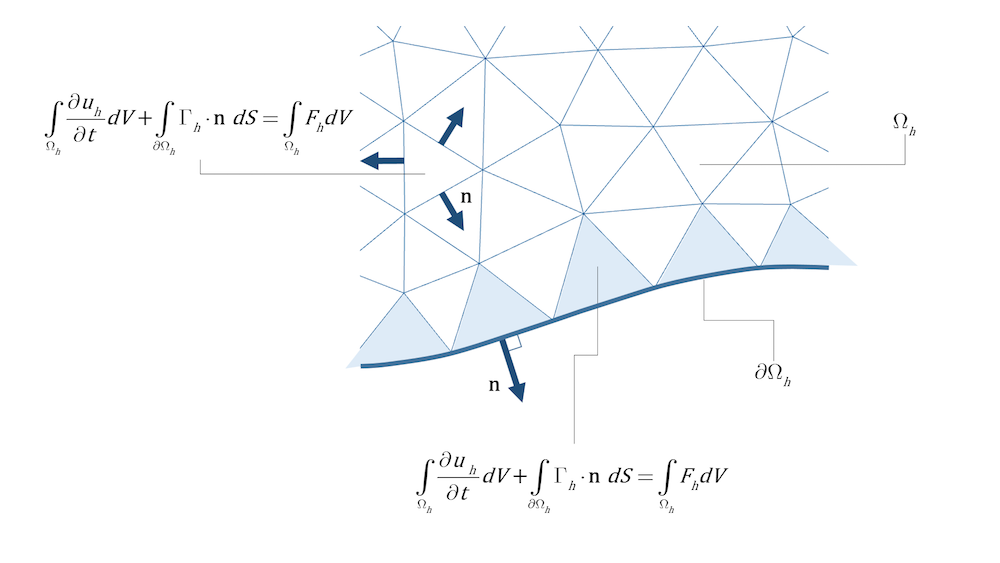
\includegraphics[width=\linewidth]{figures/integrated-flux-internal-cells.png}\\
Finite Volume Method Integration Region Diagram
\end{frame}

\begin{frame}{Principles of Finite Volume Method}
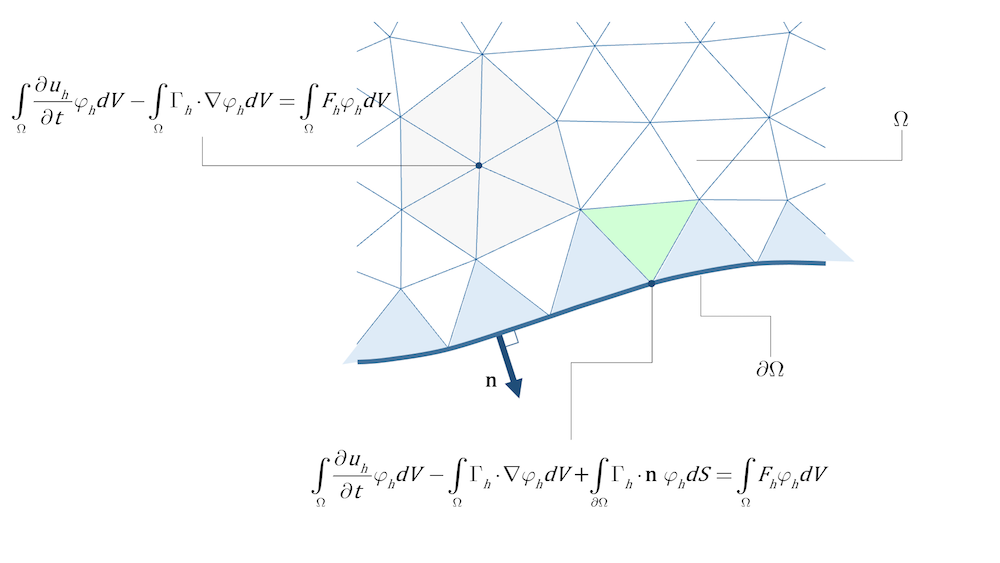
\includegraphics[width=\linewidth]{figures/domain-contribution-internal-elements.png}\\
Finite Element Method Integration Region Diagram
\end{frame}


\begin{frame}[allowframebreaks]
\frametitle{Comparison among CFD and MHD Code}
\footnotesize{\tiny}

\begin{center}
\begin{tabular}{l >{\ttfamily}c >{\ttfamily}c >{\ttfamily}c >{\ttfamily}c}
\toprule
Code & Frame & Institute & Field & Model for MHD \\
\midrule
SU2\footnote{SU2, Stanford University Unstructured \parencite{SU2EconomonIntro}} & FVM/FEM & Stanford U.(open) & CFD &-\\
JOREK & FEM & EUROfusion &   Fusion & 2-fluid \\
M3D-C1\footnote{\textcite{M3DC1:Web}} & FEM & PPPL & Fusion& 2-fluid \\
FLASH &  &  \\
PLUTO & FVM/FDTD & Torino U.(open) & Aero & 1-fluid (RMHD)\\
\bottomrule
\end{tabular}
\end{center}

\begin{center}
\begin{tabular}{l >{\ttfamily}c >{\ttfamily}c >{\ttfamily}c >{\ttfamily}c}
\toprule
Code & Grid & Adaptive Grid & $\cdots$ & $\cdots$ \\
\midrule
SU2 & Unstructured & Support \\
JOREK & Flux-aligned & - & \\
M3D-C1 & Unstructured &\\
FLASH &  &  \\
PLUTO & Structured & Support &\\
\bottomrule
\end{tabular}
\end{center}
\end{frame}

\begin{frame}{Comparison among CFD and MHD Code}
\footnotesize

The most two popular codes in CFD are (1) openFOAM and (2) SU2, in which openFOAM is too large and old for an application in the future. Considering the following points, \alert{SU2} is adopted as the final choice of my research.  

There are some requirements for the research,
\begin{description}
    \item[Modularized]The equations can be coupled flexibly. Especially for multiphysics application, e.g. the plasma-wall interaction is sometimes needed while sometimes omitted for saving time.
    \item[Modern]It would save a lot of time if no fortran embedded.
    \item[Unstructured]Due to the geometry of torus, the grid arrangement is essential for the computation accuracy. Even the flux-aligned 2D Bezier finite element in JOREK may be not precise enough to capture instabilities during the double nut merging due to the flux-aligned grid only has one center. 
    \item[Adaptive Mesh]An adaptive mesh will not only make the result more accurate, but also save tremendous computation resources from those grids which change not so quickly.
\end{description}


\end{frame}


\begin{frame}{JOREK and M3D-C1 Mesh}
\begin{figure}
\begin{minipage}[t]{0.5\linewidth}
\centering
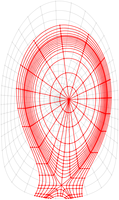
\includegraphics[width=1.2in]{figures/grid_xpoint_medium.png}
\caption{JOREK Mesh}
% \label{fig:side:a}
\end{minipage}%
\begin{minipage}[t]{0.5\linewidth}
\centering
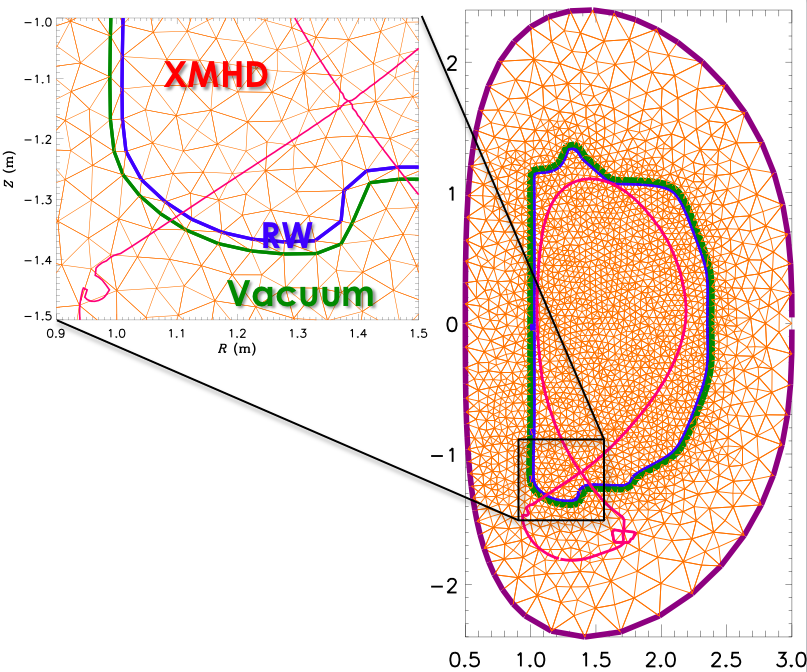
\includegraphics[width=1.8in]{figures/M3D_C1_resistive_wall.png}
\caption{M3D-C1 Mesh}
% \label{fig:side:b}
\end{minipage}
\end{figure}
    
\end{frame}

\begin{frame}{Adaptive Mesh in SU2}
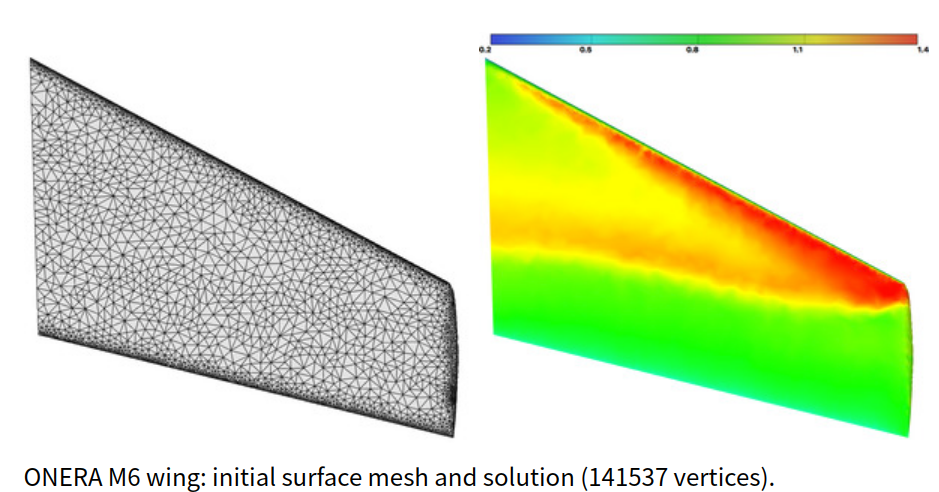
\includegraphics[width=\linewidth]{figures/ONERA_Wing_Initial_Mesh.png}
\end{frame}

\begin{frame}{Adaptive Mesh in SU2}
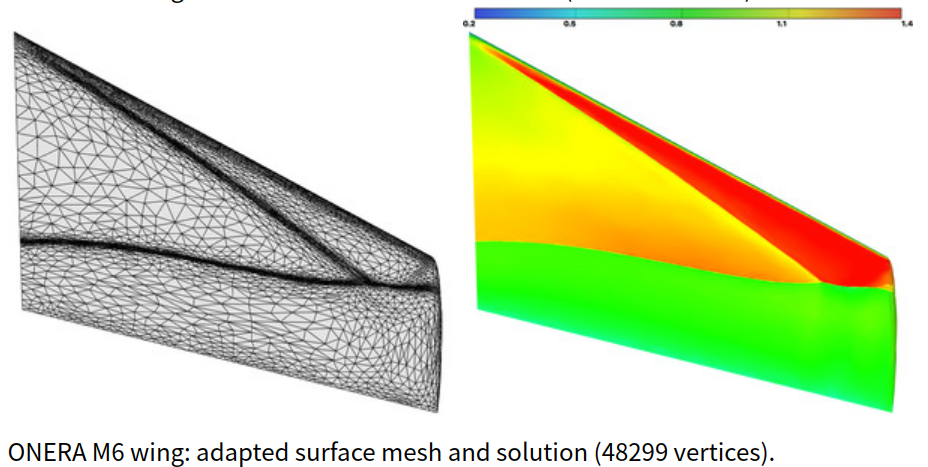
\includegraphics[width=\linewidth]{figures/ONERA_Wing_Adapted_Mesh.png}
\end{frame}

\subsection{Physics of Codes}

\begin{frame}{Physics of Codes, M3D-C1}
Firstly, a set of fluid equations,
\begin{equation}
\begin{aligned} \frac{\partial n}{\partial t}+\nabla \cdot(n \vec{u})=& 0 \\ n m_{i}\left(\frac{\partial \vec{u}}{\partial t}+\vec{u} \cdot \nabla \vec{u}\right)=& \vec{J} \times \vec{B}-\nabla p-\nabla \cdot \Pi+\vec{F} \\ \frac{\partial p}{\partial t}+\vec{u} \cdot \nabla p+\Gamma p \nabla \cdot \vec{u}=&(\Gamma-1)\left[Q-\nabla \cdot \vec{q}+\eta J^{2}-\vec{u} \cdot \vec{F}-\Pi : \nabla u\right] \\ &+\frac{1}{n e} \vec{J} \cdot\left(\frac{\nabla n}{n} p_{e}-\nabla p_{e}\right)+(\Gamma-1) \Pi_{e} : \nabla\left(\frac{1}{n e} \vec{J}\right) \\ \frac{\partial p_{e}}{\partial t}+\vec{u} \cdot \nabla p_{e}+\Gamma p_{e} \nabla \cdot \vec{u}=&(\Gamma-1)\left[Q_{e}-\vec{q}_{e}+\eta J^{2}-\vec{u} \cdot \vec{F}_{e}-\Pi_{e} : \nabla u\right] \\ &+\frac{1}{n e} \vec{J} \cdot\left(\frac{\nabla n}{n} p_{e}-\nabla p_{e}\right)+(\Gamma-1)\left[\Pi_{e} : \nabla\left(\frac{1}{n e} \vec{J}\right)+\frac{1}{n e} \vec{J} \cdot \vec{F}_{e}\right] \end{aligned}
\end{equation}

Generalized Ohm's law,
\begin{equation}
\vec{E}=-\vec{u} \times \vec{B}+\eta \vec{J}+\frac{1}{n e}\left(\vec{J} \times \vec{B}-\nabla p_{e}-\nabla \cdot \Pi_{e}+\vec{F}_{e}\right)
\end{equation}

A reduced set of Maxwell's equations,
\begin{equation}
\begin{aligned} \vec{J} &=\frac{1}{\mu_{0}} \nabla \times \vec{B} \\ \frac{\partial \vec{B}}{\partial t} &=-\nabla \times \vec{E} \end{aligned}
\end{equation}
\end{frame}

\begin{frame}{Physics of Codes, JOREK}

2-fluid MHD model is probably a too large topic to talk about in this presentation, because it is not the focus of the presentation.

Here we have the resitivity MHD model in JOREK as an example.

\alert{Resitivity MHD model},
\begin{equation}
\left\{
\begin{array}{l}
{\partial_{t} \rho+\nabla \cdot(\rho \boldsymbol{v})=0} \\ 
{\rho \partial_{t} \boldsymbol{v}+\rho \boldsymbol{v} \cdot \nabla \boldsymbol{v}+\nabla(p)=\boldsymbol{J} \times \boldsymbol{B}+\nabla \cdot(\nu \nabla \boldsymbol{v})} \\ 
{\partial_{t} p+\boldsymbol{v} \cdot \nabla p+\gamma p \nabla \cdot \boldsymbol{v}=0} \\ {\partial_{t} \boldsymbol{B}=-\nabla \times \boldsymbol{E}=\nabla \times(\boldsymbol{v} \times \boldsymbol{B}-\eta \boldsymbol{J})} \\ {\nabla \times \boldsymbol{B}=\boldsymbol{J}} \\ {\nabla \cdot \boldsymbol{B}=0}\end{array}\right.
\end{equation}

Be careful of the degenerative Maxwell:
\begin{itemize}
    \item $\boldsymbol{J}$ is decided by the curl of magnetic field here, which means $\boldsymbol{E}$ is much more stable than $\boldsymbol{B}$.
    \item Time derivative of $p$ is replaced by the energy derivative in fluid dynamics SU2. 
\end{itemize}


\end{frame}


\begin{frame}{Physics of Codes, SU2}


\begin{equation*}
\frac{\partial U}{\partial t}+\nabla \cdot \vec{F}^{c}-\nabla \cdot\left(\mu^{v k} \vec{F}^{v k}\right)=Q \quad \text { in } \Omega, t>0
\end{equation*}


\begin{equation*}
U=\left\{\begin{array}{c}{\rho } \\ {\rho \vec{v} } \\ {\rho E}\end{array}\right\},\quad
\vec{F}^{c}=\left\{\begin{array}{c}{\rho \vec{v}} \\ {\rho \vec{v} \otimes \vec{v}+\overline{\overline{I}} p} \\ {\rho E \vec{v}+p \vec{v}}\end{array}\right\}
\end{equation*}

\begin{equation*}
\vec{F}^{v1}=\left\{\begin{array}{c}{\cdot} \\ {\overline{\overline{\tau}}} \\ {\overline{\overline{\tau}}\cdot \vec{v}}\end{array}\right\},\quad
\vec{F}^{v2}=\left\{\begin{array}{c}{\cdot} \\ {\cdot} \\ {c_p \nabla T}\end{array}\right\},\quad
Q=\left\{\begin{array}{c}{q_\rho} \\ {\vec{q}_{\rho\vec{v}}} \\ {q_{\rho E}}\end{array}\right\}
\end{equation*}

\end{frame}

\begin{frame}{Conservative Equations}
\begin{equation}
\frac{\partial \boldsymbol{U}}{\partial t}+\underbrace{\nabla \cdot \boldsymbol{F}^{c}}_{\text CONV\ TERM}-\overbrace{\nabla \cdot\left(\mu^{v k} \boldsymbol{F}^{v k}\right)}^{\text VISC\ TERM}=\boldsymbol{Q} \quad \text { in }\Omega,  \quad t>0
\end{equation}

Most SU2 scripts are located in the \textit{SU2\_CFD} and \textit{Common} folder, other folders contain very limited amount of codes concerning adaptive mesh, dual grid and \textit{e.t.c.} 

\begin{itemize}
    \item OS: Cross-platform
    \item Lang: C++, Python
    \item Mainly vertex-based dual mesh FVM, also supports FEM and primal grid
\end{itemize}
\end{frame}

\begin{frame}{SU2 Framework}
\uncover<+->{\begin{equation*}
\frac{\partial U}{\partial t}+\nabla \cdot \vec{F}^{c}-\nabla \cdot\left(\mu^{v k} \vec{F}^{v k}\right)=Q \quad \text { in } \Omega, t>0
\end{equation*}
}
\uncover<+->{\[ \Downarrow \]
\begin{align*}
    \int_{\Omega_{i}} \frac{\partial U}{\partial t} d \Omega & + \sum_{j \in \mathcal{N}(i)}\left(\tilde{F}_{i j}^{c}+\tilde{F}_{i j}^{v k}\right) \Delta S_{i j}-Q\left|\Omega_{i}\right| \\ 
=\int_{\Omega_{i}} \frac{\partial U}{\partial t} d \Omega & +  R_{i}(U)=0
\end{align*}
}

For each variable in each cell, there is a residual.
\end{frame}



% \subsection{Temporal Discretization}
\begin{frame}{Temporal Discretization}
The requirement of temporal discretization in Maxwell equations is no different from others.

Explicit RK,
\begin{equation}
\left\{\begin{array}{l}{u^{(1)}=u^{n}} \\ {u^{(2)}=u^{n}+\alpha_{2} d t F\left(u^{(1)}\right)} \\ {u^{(3)}=u^{n}+\alpha_{3} d t F\left(u^{(2)}\right)} \\ {\cdots} \\ {u^{(k)}=u^{n}+\alpha_{k} d t F\left(u^{(k-1)}\right)} \\ {u^{n+1}=u^{n}+d t \sum_{j=1}^{q} \beta_{j} F\left(u^{(j)}\right)}\end{array}\right.
\end{equation}

Implicit RK and dual time stepping \parencite{SU2LiDualTime} are also available in SU2, and compatible with the Maxwell equations.
\end{frame}





% \begin{frame}[fragile,allowframebreaks]
% \frametitle{Java Code Sample}
    
% \begin{lstlisting}[language=Java,basicstyle=\ttfamily\footnotesize,gobble=8,
%     emph={parse,lp,typedDependenciesCCprocessed,lemmaStatic,dep,gov,reln,index,tag,value},
%     morekeywords={TreebankLanguagePack,GrammaticalStructureFactory,GrammaticalStructure,
%         List,TypedDependency,IndexedWord,String,Morphology},
%         escapechar=|]
%         // Continue from earlier Java code 
%         // Use the parsed tree to get the typed dependencies
%         TreebankLanguagePack tlp = lp.treebankLanguagePack();
%         GrammaticalStructureFactory gsf = tlp.grammaticalStructureFactory();
%         GrammaticalStructure gs = gsf.newGrammaticalStructure(parse);
%         List<TypedDependency> tdl = gs.typedDependenciesCCprocessed();

%         // Let's just print out each of the parent-child relationship first
%         for (TypedDependency td : tdl) {
%             // parent = "governer"
%             IndexedWord parent = td.gov();
%             String parentWord = parent.value();
%             String parentPOS = parent.tag();
%             String parentLemma = Morphology.lemmaStatic(
%                 parentWord, parentPOS, true);
            
%             |\framebreak|
%             // child = "dependent"
%             IndexedWord child = td.dep();
%             String childWord = child.value();
%             String childPOS = child.tag();
%             String childLemma = Morphology.lemmaStatic(
%                 childWord, childPOS, true);
            
            
%             System.out.println(
%                 "[" + parent.index() + "]" + parentLemma + "/" + parentPOS 
%                 + " <--" + td.reln().getShortName() + "-- "
%                 + "[" + child.index() + "]" + childLemma + "/" + childPOS);
%         }
%         System.out.println();
% \end{lstlisting}

% \end{frame}








\begin{frame}{Vertex-based Dual Grid}
\begin{figure}
    \centering
    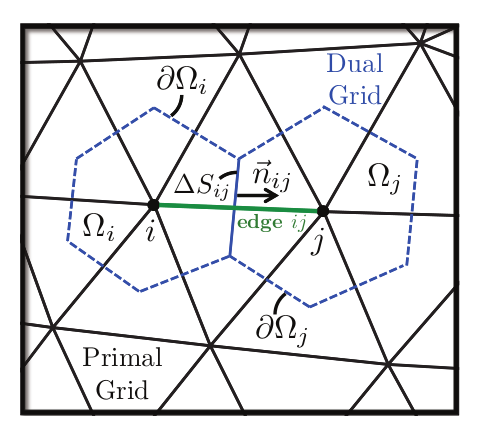
\includegraphics[width=0.5\linewidth]{figures/DualMeshControlVolume.png}
    \caption{Dual mesh control volumes surrounding two nodes, $i$ and $j$, in the domain interior.}
    % \label{fig:my_label}
\end{figure}


By virtue of the functionality of geometry-relevant source, researchers do not need to implement the area calculation step and are capable to use the face area and normal vector directly.

\end{frame}

%!TEX root = Intro-NLP-seminar.tex

\section{Maxwell Equations in FVM}

% \subsection{Denotations and Equations used in Maxwell-FVM}
\begin{frame}{Maxwell Equations}
Maxwell equations indicate that the $\boldsymbol{E}$ and $\boldsymbol{H}$ changes are decided by the curl of the other variable. \parencite{rao1999time} That is unprecedented in other fluid equations, which brings new numerical trouble.

\begin{equation}
\left\{\begin{array}{l}{\nabla \times \boldsymbol{H}-\varepsilon \frac{\partial \boldsymbol{E}}{\partial t}-\sigma \boldsymbol{E}=\boldsymbol{J}} \\ {\nabla \times \boldsymbol{E}+\mu \frac{\partial \boldsymbol{H}}{\partial t}=\boldsymbol{K}}\end{array}\right.
\end{equation}

The following continuity conditions always work for any interface,

\begin{equation}
\begin{array}{r}{\left[\boldsymbol{E}_{\mathrm{\tau}}, \boldsymbol{H}_{\mathrm{\tau}}\right]_{-}^{+}=0} \\ {\left[\varepsilon \boldsymbol{a}_{\mathrm{n}} \cdot \boldsymbol{E}, \mu \boldsymbol{a}_{\mathrm{n}} \cdot \boldsymbol{H}\right]_{-}^{+}=0}\end{array}
\end{equation}

The $[\ \cdot\ ]^+_-$ symbols mean the difference between the positive side of the interface and the negative.

\end{frame}

% \begin{frame}{Maxwell Equations}

% In the special cases of impenetrable obstacles, one would take $\boldsymbol{e} = 0$ on perfect conductors and $\boldsymbol{h} = 0$ on perfectly magnetizable media, respectively.

% \begin{equation}
% \left\{\begin{array}{l}{\left.\boldsymbol{E}_{\mathrm{\tau}}\right|_{\partial \Omega}=\boldsymbol{e}} \\ {\left.\boldsymbol{H}_{\mathrm{\tau}}\right|_{\partial \Omega}=\boldsymbol{h}}\end{array}\right.
% \end{equation}

% The $\boldsymbol{e} = 0$ boundary condition is a common one in electromagnetic simulation, but primitive. More advanced boundary to simulate far-field condition will be illustrated subsequently.

% \end{frame}

% \begin{frame}{Maxwell Equations}

% For convenience to do computation, $s$ is denoted as a function mapping a vector to an antisymmetric 3 x 3 matrices.
% \begin{equation}
% s : R^{3} \rightarrow \Lambda^{2}\left(R^{3}\right)
% \end{equation}


% \begin{equation}
% s :\left(v_{1}, v_{2}, v_{3}\right) \longmapsto\left[\begin{array}{ccc}{0} & {-v_{3}} & {v_{2}} \\ {v_{3}} & {0} & {-v_{1}} \\ {-v_{2}} & {v_{1}} & {0}\end{array}\right]
% \end{equation}

% Special divergence is also defined, for handling the divergence of a 'matrix'.
% \begin{equation}
% [\operatorname{Div}(s(\boldsymbol{V}))]_{q}=\sum_{p=1}^{3} \frac{\partial}{\partial x^{p}}[s(\boldsymbol{V})]_{p q}
% \end{equation}


% \end{frame}

% \begin{frame}{Maxwell Equations}
% There are two essential characteristics of this funciton.

% Firstly, to calculate the curl of a vector-value variable by a divergence operator is not availiable. 
% \begin{equation}
% \operatorname{Div}(s(\boldsymbol{V}))=\nabla \times \boldsymbol{V}
% \end{equation}


% Secondly, it makes it easier to do cross-product.
% \begin{equation}
% s(\boldsymbol{a}_n)\boldsymbol{V}= \boldsymbol{a}_n \times \boldsymbol{V}
% \end{equation}


% \end{frame}



% \begin{frame}{Maxwell Equations}
% \begin{equation}
% \left\{\begin{array}{l}{\varepsilon \frac{\partial \boldsymbol{E}}{\partial t}-\operatorname{Div}(s(\boldsymbol{H}))+\sigma \boldsymbol{E}=-\boldsymbol{J}} \\ {\mu \frac{\partial \boldsymbol{H}}{\partial t}+\operatorname{Div}(s(\boldsymbol{E}))=\boldsymbol{K}}\end{array}\right.
% \end{equation}


% \begin{equation}
% \alpha \frac{\partial \boldsymbol{U}}{\partial t}+\operatorname{div}(\mathcal{A} \boldsymbol{U})+\mathcal{B} \boldsymbol{U}=\boldsymbol{G}
% \end{equation}

% Attention, the $\operatorname{div}$ operates on each row of 6 x 3 matrix and acquire a 6 x 1 vector, different from the $\operatorname{Div}$ operator.

% \begin{equation}
% \begin{array}{c}{[\alpha]=\left[\begin{array}{cc}{\varepsilon} & {0} \\ {0} & {\mu}\end{array}\right] \quad[\mathcal{A}]=\left[\begin{array}{cc}{0} & {-s(\cdot)} \\ {s(\cdot)} & {0}\end{array}\right] \quad[\mathcal{B}]=\left[\begin{array}{cc}{\sigma} & {0} \\ {0} & {0}\end{array}\right]} \\ {\boldsymbol{G}=\left[\begin{array}{c}{-\boldsymbol{J}} \\ {\boldsymbol{K}}\end{array}\right]}\end{array}
% \end{equation}

% \begin{equation}
% \mathcal{A} U=F(U)=\left(F_{1}(U) ; F_{2}(U) ; F_{3}(U)\right)
% \end{equation}

% \end{frame}

% \begin{frame}{Maxwell Equation, Spatial Discretization}
% Let's put the current density aside, which is not a big problem after the integration.

% Then it becomes the \alert{Conservative Form Maxwell equations}:

% \begin{equation}
% \begin{aligned} \varepsilon \frac{\partial \boldsymbol{E}}{\partial t}-\nabla \times \boldsymbol{H} &=0 \\ \mu \frac{\partial \boldsymbol{H}}{\partial t}+\nabla \times \boldsymbol{E} &=0 \end{aligned}
% \end{equation}



% \begin{equation}
% \mathcal{A} \boldsymbol{U}=F(\boldsymbol{U})=\left(F_{1}(\boldsymbol{U}) ; F_{2}(\boldsymbol{U}) ; F_{3}(\boldsymbol{U})\right)
% \end{equation}

% \end{frame}



% \begin{frame}{Maxwell Equations}
% \begin{equation}
% F_{1}(\boldsymbol{U})=\left[\begin{array}{c}{0} \\ {H_{2}} \\ {-H_{y}} \\ {0} \\ {-E_{z}} \\ {E_{y}}\end{array}\right] \quad F_{2}(\boldsymbol{U})=\left[\begin{array}{c}{-H_{z}} \\ {0} \\ {H_{x}} \\ {E_{z}} \\ {0} \\ {-E_{x}}\end{array}\right] \quad F_{3}(\boldsymbol{U})=\left[\begin{array}{c}{H_{y}} \\ {-H_{x}} \\ {0} \\ {-E_{y}} \\ {E_{x}} \\ {0}\end{array}\right]
% \end{equation}

% \begin{equation}
% \alpha \frac{\partial \boldsymbol{U}}{\partial t}+\frac{\partial F_{1}(\boldsymbol{U})}{\partial x}+\frac{\partial F_{2}(\boldsymbol{U})}{\partial y}+\frac{\partial F_{3}(\boldsymbol{U})}{\partial z}=0
% \end{equation}

% \begin{equation}
% \alpha \frac{\partial \boldsymbol{U}}{\partial t}+\operatorname{div} F(\boldsymbol{U})=0
% \end{equation}

% \end{frame}

\begin{frame}{Maxwell Equation, Spatial Discretization}

\begin{equation}
\alpha \int_{V} \frac{\partial \boldsymbol{U}}{\partial t} d V+\int_{V} \operatorname{div} F(\boldsymbol{U}) d \boldsymbol{V}=0
\end{equation}

\begin{equation}
\frac{\partial \boldsymbol{U}_{i}}{\partial t}=-\frac{1}{\left|V_{i}\right|} \sum_{k\in\mathcal{N}_i}\left|S_{k}\right| \alpha^{-1} F\left(\boldsymbol{U}_{k}^{*}\right) \cdot \boldsymbol{a}_{\mathrm{nk}}
\end{equation}

\begin{equation}
F\left(\boldsymbol{U}_{k}^{*}\right) \cdot \boldsymbol{a}_{n k}=\left[\begin{array}{c}{-\boldsymbol{a}_{n k} \times \boldsymbol{H}_{k}^{*}} \\ {\boldsymbol{a}_{n k} \times \boldsymbol{E}_{k}^{*}}\end{array}\right]
\end{equation}
    
The spatial discretization methods focus on the key variable, $F\left(\boldsymbol{U}_{k}^{*}\right) \cdot \boldsymbol{a}_{\mathrm{nk}}$. How to accurately compute the value of the flux is the kernel of FVM, that is, computing the $\boldsymbol{a}_{n k} \times \boldsymbol{H}_{k}^{*}, \boldsymbol{a}_{n k} \times \boldsymbol{E}_{k}^{*}$.
\end{frame}

% \subsection{How to Compute the Flux in Maxwell Equations}
\begin{frame}{$F\left(\boldsymbol{U}_{k}^{*}\right) \cdot \boldsymbol{a}_{\mathrm{nk}}$}
How to calculate the flux, $F\left(\boldsymbol{U}_{k}^{*}\right) \cdot \boldsymbol{a}_{\mathrm{nk}}$? The values on the cell boundary are needed, but we only store the values on the nodes.

Then one might come up with these ideas,

\begin{description}
\item[\textbf{Interpolation}] By utility of the value interpolation from the values at adjacent nodes, the flux is easy to get and have a high-order accuracy. It would be quite useful for the continuously differentiable functions but probably not for $\varepsilon$ or $\mu$ on the boundary of materials. 
\item[\textbf{Flux-Splitting}] To settle the problem arising from numerical instability of other methods, flux-splitting method is used.
\end{description}
The following content related to the flux-splitting method begins with a matrix constructed by the $\boldsymbol{a}_{\mathrm{n}}$.

\end{frame}

\begin{frame}{$F\left(\boldsymbol{U}_{k}^{*}\right) \cdot \boldsymbol{a}_{\mathrm{nk}}$, $A$ Matrix}
One can use the normal vectors of a cell's faces to represent the local coordinates, as a basis of coordinate,
\begin{equation}
R^{m_{i}} \ni\left(\xi_{1}, \cdots, \xi_{m_{i}}\right) \mapsto x=\sum_{k=1}^{m_{i}} \xi_{k} a_{\mathrm{nk}} \in R^{3}
\end{equation}

\begin{equation}
\frac{\partial \boldsymbol{U}}{\partial t}=-\alpha^{-1} \sum_{k=1}^{m_{i}}\left(\frac{\partial F_{1}}{\partial \boldsymbol{U}} \frac{\partial \xi_{k}}{\partial x}+\frac{\partial F_{2}}{\partial \boldsymbol{U}} \frac{\partial \xi_{k}}{\partial y}+\frac{\partial F_{3}}{\partial \boldsymbol{U}} \frac{\partial \xi_{k}}{\partial z}\right) \frac{\partial \boldsymbol{U}}{\partial \xi_{k}}
\end{equation}
\begin{equation}
\frac{\partial \boldsymbol{U}}{\partial t}=-\alpha^{-1} \sum_{k=1}^{m_{i}} A\left(\boldsymbol{a}_{\mathrm{nk}}\right) \frac{\partial \boldsymbol{U}}{\partial n_{k}}
\end{equation}
\end{frame}


\begin{frame}{$F\left(\boldsymbol{U}_{k}^{*}\right) \cdot \boldsymbol{a}_{\mathrm{nk}}$, $A$ Matrix}
\begin{equation}
A\left(\boldsymbol{a}_{\mathrm{n}}\right)=\left[\begin{array}{cccccc}{0} & {0} & {0} & {0} & {n_{z}} & {-n_{y}} \\ {0} & {0} & {0} & {-n_{z}} & {0} & {n_{x}} \\ {0} & {0} & {0} & {n_{y}} & {-n_{x}} & {0} \\ {0} & {-n_{z}} & {n_{y}} & {0} & {0} & {0} \\ {n_{z}} & {0} & {-n_{x}} & {0} & {0} & {0} \\ {-n_{y}} & {n_{x}} & {0} & {0} & {0} & {0}\end{array}\right]
\end{equation}

\begin{equation}
\tilde{A}\left(\boldsymbol{a}_{\mathrm{n}}\right)=\alpha^{-1} A\left(\boldsymbol{a}_{\mathrm{n}}\right)=P\ \Lambda\ P^{-1},
\end{equation}

with six eigenvalues also as the diagonal of $\Lambda$
\begin{equation}
\Lambda = diag \left(0,0, \frac{1}{\sqrt{\mu \varepsilon}}, \frac{1}{\sqrt{\mu \varepsilon}},-\frac{1}{\sqrt{\mu \varepsilon}},-\frac{1}{\sqrt{\mu \varepsilon}}\right) = diag \left(0,0,v,v,-v,-v\right),
\end{equation}
where $v$ is the light speed in the medium. 
\end{frame}

\begin{frame}{Maxwell Equations}

For convenience to do computation, $s$ is denoted as a function mapping a vector to an antisymmetric 3 x 3 matrices.
\begin{equation}
s : R^{3} \rightarrow \Lambda^{2}\left(R^{3}\right)
\end{equation}


\begin{equation}
s :\left(v_{1}, v_{2}, v_{3}\right) \longmapsto\left[\begin{array}{ccc}{0} & {-v_{3}} & {v_{2}} \\ {v_{3}} & {0} & {-v_{1}} \\ {-v_{2}} & {v_{1}} & {0}\end{array}\right]
\end{equation}

Special divergence is also defined, for handling the divergence of a 'matrix'.
\begin{equation}
[\operatorname{Div}(s(\boldsymbol{V}))]_{q}=\sum_{p=1}^{3} \frac{\partial}{\partial x^{p}}[s(\boldsymbol{V})]_{p q}
\end{equation}


\end{frame}

\begin{frame}{Maxwell Equations}
There are two essential characteristics of this funciton.

Firstly, to calculate the curl of a vector-value variable by a divergence operator is not availiable. 
\begin{equation}
\operatorname{Div}(s(\boldsymbol{V}))=\nabla \times \boldsymbol{V}
\end{equation}


Secondly, it makes it easier to do cross-product.
\begin{equation}
s(\boldsymbol{a}_n)\boldsymbol{V}= \boldsymbol{a}_n \times \boldsymbol{V}
\end{equation}


\end{frame}
\begin{frame}{$F\left(\boldsymbol{U}_{k}^{*}\right) \cdot \boldsymbol{a}_{\mathrm{nk}}$, $A$ Matrix}
\begin{equation}
P=\left[\begin{array}{cccccc}{n_{x}} & {0} & {\frac{n_{x} n_{z}}{v \varepsilon}} & {-\frac{n_{x} n_{y}}{v \varepsilon}} & {-\frac{n_{x} n_{z}}{v \varepsilon}} & {\frac{n_{x} n_{y}}{v \varepsilon}} \\ {n_{y}} & {0} & {\frac{n_{y} n_{z}}{v \varepsilon}} & {\frac{n_{x}^{2}+n_{z}^{2}}{v \varepsilon}} & {-\frac{n_{y} n_{z}}{v \varepsilon}} & {-\frac{n_{x}^{2}+n_{z}^{2}}{v \varepsilon}} \\ {n_{z}} & {0} & {-\frac{n_{x}^{2}+n_{y}^{2}}{v \varepsilon}} & {-\frac{n_{y} n_{z}}{v \varepsilon}} & {\frac{n_{x}^{2}+n_{y}^{2}}{v \varepsilon}} & {\frac{n_{y} n_{z}}{v \varepsilon}} \\ {0} & {n_{x}} & {-n_{y}} & {-n_{z}} & {-n_{y}} & {-n_{z}} \\ {0} & {n_{y}} & {n_{x}} & {0} & {n_{x}} & {0} \\ {0} & {n_{z}} & {0} & {n_{x}} & {0} & {n_{x}}\end{array}\right]
\end{equation}

If we consider the variation of U to be only with respect to the $\tilde{A}\left(\boldsymbol{a}_{\mathrm{n}}\right)$ direction, then equation simplies to,
\begin{equation}
\frac{\partial \boldsymbol{U}}{\partial t}=-\tilde{A}\left(\boldsymbol{a}_{\mathrm{n}}\right) \frac{\partial \boldsymbol{U}}{\partial n}
\end{equation}

Using the previous decomposition of $\tilde{A}\left(\boldsymbol{a}_{\mathrm{n}}\right)$ and introducing the vector $V = P^{-1}U$
\begin{equation}
\frac{\partial V_{j}}{\partial t}+\lambda_{j} \frac{\partial V_{j}}{\partial n}=0 \quad j=1, \cdots, 6
\end{equation}

\end{frame}

\begin{frame}{Maxwell Equations, Flux-Splitting}
\begin{equation}
V_{j}(\xi, t)=f\left(\lambda_{j} t-\xi n\right),
\end{equation}
\begin{equation}
V_{j}\left(\xi_{0}, t-\frac{d}{\lambda_{j}}\right)=V_{j}\left(\xi^{*}, t\right)
\end{equation}

A crude approximation would be like the following.
\begin{equation}\label{VApproxBoundary}
V_{j}(t)=V_{j}^{*}(t)
\end{equation}

\begin{equation}
\tilde{A}\left(\boldsymbol{a}_{\mathrm{n}}\right)=P \Lambda P^{-1}=P\left(\Lambda^{+}+\Lambda^{-}\right) P^{-1}=P \Lambda^{+} P^{-1}+P \Lambda^{-} P^{-1}=\tilde{A}\left(\boldsymbol{a}_{\mathrm{n}}\right)^{+}+\tilde{A}\left(\boldsymbol{a}_{\mathrm{n}}\right)^{-}
\end{equation}

Multiply both sides of equation (\ref{VApproxBoundary}) by $P\Lambda^+$
\begin{equation}
\tilde{A}\left(\boldsymbol{a}_{\mathrm{n}}\right)^{+} \boldsymbol{U}=\tilde{A}\left(\boldsymbol{a}_{\mathrm{n}}\right)^{+} \boldsymbol{U}^{*}
\end{equation}
\end{frame}

\begin{frame}{Maxwell Equations, Flux-Splitting}
\tiny
\begin{equation}
\tilde{A}\left(\boldsymbol{a}_{\mathrm{n}}\right)^{+}=\frac{1}{2}\left[\begin{array}{cccccc}{\left(n_{z}^{2}+n_{y}^{2}\right) v} & {-n_{x} n_{y} v} & {-n_{x} n_{z} v} & {0} & {n_{z} \frac{1}{\varepsilon}} & {-n_{y} \frac{1}{\varepsilon}} \\ {-n_{x} n_{y} v} & {\left(n_{x}^{2}+n_{z}^{2}\right) v} & {-n_{y} n_{z} v} & {-n_{z} \frac{1}{\varepsilon}} & {0} & {n_{x} \frac{1}{\varepsilon}} \\ {-n_{x} n_{z} v} & {-n_{y} n_{z} v} & {\left(n_{x}^{2}+n_{y}^{2}\right) v} & {n_{y} \frac{1}{\varepsilon}} & {-n_{x} \frac{1}{\varepsilon}} & {0} \\ {0} & {-n_{z} \frac{1}{\mu}} & {n_{y} \frac{1}{\mu}} & {\left(n_{z}^{2}+n_{y}^{2}\right) v} & {-n_{x} n_{y} v} & {-n_{x} n_{z} v} \\ {n_{z} \frac{1}{\mu}} & {0} & {-n_{x} \frac{1}{\mu}} & {-n_{x} n_{y} v} & {\left(n_{x}^{2}+n_{z}^{2}\right) v} & {-n_{y} n_{z} v} \\ {-n_{y} \frac{1}{\mu}} & {n_{x} \frac{1}{\mu}} & {0} & {-n_{x} n_{z} v} & {-n_{y} n_{z} v} & {\left(n_{x}^{2}+n_{y}^{2}\right) v}\end{array}\right]
\end{equation}
\normalsize

\begin{equation}
\tilde{A}\left(\boldsymbol{a}_{\mathrm{n}}\right)^{-}=-\tilde{A}\left(-\boldsymbol{a}_{\mathrm{n}}\right)^{+}
\end{equation}

\begin{equation}
\tilde{A}\left(\boldsymbol{a}_{\mathrm{n}}\right)^{+}=\frac{1}{2}\begin{bmatrix}
-vs^2(\boldsymbol{a}_n) & \frac{-1}{\varepsilon} s(\boldsymbol{a}_n) \\ 
\frac{1}{\mu} s(\boldsymbol{a}_n) & -vs^2(\boldsymbol{a}_n
\end{bmatrix},\quad \tilde{A}\left(\boldsymbol{a}_{\mathrm{n}}\right)^{+} \boldsymbol{U}=\tilde{A}\left(\boldsymbol{a}_{\mathrm{n}}\right)^{+} \boldsymbol{U}^{*}
\end{equation}




\begin{equation}
Y=\sqrt{\frac{\varepsilon}{\mu}}, Z=\sqrt{\frac{\mu}{\varepsilon}}
\end{equation}
\end{frame}


\begin{frame}{Maxwell Equations, Flux-Splitting}
For \textbf{dielectric contrast},
\begin{equation}
\left\{\begin{array}{l}{\boldsymbol{a}_{\mathbf{n}} \times \boldsymbol{E}^{*}=\boldsymbol{a}_{\mathbf{n}} \times \boldsymbol{E}^{* *}} \\ {\boldsymbol{a}_{\mathbf{n}} \times \boldsymbol{H}^{*}=\boldsymbol{a}_{\mathbf{n}} \times \boldsymbol{H}^{* *}}\end{array}\right.
\end{equation}


\begin{equation}
\left\{\begin{array}{l}{Y^{\mathrm{L}} \boldsymbol{a}_{\mathrm{n}} \times \boldsymbol{E}^{*}-\boldsymbol{a}_{\mathrm{n}} \times\left(\boldsymbol{a}_{\mathrm{n}} \times \boldsymbol{H}^{*}\right)=Y^{\mathrm{L}} \boldsymbol{a}_{\mathrm{n}} \times \boldsymbol{E}^{\mathrm{L}}-\boldsymbol{a}_{\mathrm{n}} \times\left(\boldsymbol{a}_{\mathrm{n}} \times \boldsymbol{H}^{\mathrm{L}}\right)} \\ {Y^{\mathrm{R}} \boldsymbol{a}_{\mathrm{n}} \times \boldsymbol{E}^{* *}+\boldsymbol{a}_{\mathrm{n}} \times\left(\boldsymbol{a}_{\mathrm{n}} \times \boldsymbol{H}^{* *}\right)=Y^{\mathrm{R}} \boldsymbol{a}_{\mathrm{n}} \times \boldsymbol{E}^{\mathrm{R}}+\boldsymbol{a}_{\mathrm{n}} \times\left(\boldsymbol{a}_{\mathrm{n}} \times \boldsymbol{H}^{\mathrm{R}}\right)}\end{array}\right.
\end{equation}


\begin{equation}
F\left(\boldsymbol{U}^{*}\right) \cdot \boldsymbol{a}_{\mathrm{n}}=F\left(\boldsymbol{U}^{* *}\right) \cdot \boldsymbol{a}_{\mathrm{n}}=\alpha^{\mathrm{L}} T^{\mathrm{L}} \tilde{A}^{\mathrm{L}}\left(\boldsymbol{a}_{\mathrm{n}}\right)^{+} U^{\mathrm{L}}+\alpha^{\mathrm{R}} T^{\mathrm{R}} \tilde{A}^{\mathrm{R}}\left(\boldsymbol{a}_{\mathrm{n}}\right)^{-} \boldsymbol{U}^{\mathrm{R}}
\end{equation}

\begin{equation}
T^{\mathrm{L}, \mathrm{R}}=\left[\begin{array}{cc}{\frac{2 Z^{\mathrm{L} \cdot R}}{Z^{\mathrm{L}}+Z^{\mathrm{R}}}} & {0} \\ {0} & {\frac{2 Y^{L, R}}{Y^{\mathrm{L}}+Y^{\mathrm{R}}}}\end{array}\right]
\end{equation}





\end{frame}

\begin{frame}{Maxwell Equations, Flux-Splitting}
\begin{equation}
\alpha \frac{\partial U_{i}}{\partial t}=\frac{-1}{\left|V_{i}\right|} \sum_{k\in\mathcal{N}_i}\left|S_{k}\right|\left[\alpha^{\mathrm{L}} T^{\mathrm{L}} \tilde{A}^{\mathrm{L}}\left(\boldsymbol{a}_{\mathrm{n} k}\right)^{+} U_{k^{-}}+\alpha^{\mathrm{R}} T^{\mathrm{R}} \tilde{A}^{\mathrm{R}}\left(\boldsymbol{a}_{\mathrm{nk}}\right)^{-} U_{k^{+}}\right]
\end{equation}

If both sides' permittivity and peameability are similar such that the error could be omitted, the formula turns out to be,
\begin{equation}
\frac{\partial U_{i}}{\partial t}=\frac{-1}{\left|V_{i}\right|} \sum_{k\in\mathcal{N}_i}\left|S_{k}\right|\left[\tilde{A}\left(\boldsymbol{a}_{\mathrm{nk}}\right)^{+} U_{k^{-}}+\tilde{A}\left(\boldsymbol{a}_{\mathrm{nk}}\right)^{-} U_{k^{+}}\right]
\end{equation}
\end{frame}

\begin{frame}{Maxwell Equations, Flux-Splitting}
For \textbf{perfect conductor},
\begin{equation}
\boldsymbol{a}_{\mathrm{n}} \times \boldsymbol{E}^{*}=0
\end{equation}

\begin{equation}
\boldsymbol{a}_{\mathrm{n}} \times \boldsymbol{H}^{*}=Y \boldsymbol{a}_{\mathrm{n}} \times\left(\boldsymbol{a}_{\mathrm{n}} \times \boldsymbol{E}\right)+\boldsymbol{a}_{\mathrm{n}} \times \boldsymbol{H}
\end{equation}

\begin{equation}
F\left(\boldsymbol{U}^{*}\right) \cdot \boldsymbol{a}_{\mathrm{n}}=\alpha^{\mathrm{L}} T_{p c}^{\mathrm{L}} \tilde{A}^{\mathrm{L}}\left(\boldsymbol{a}_{\mathrm{n}}\right)^{+} \boldsymbol{U}^{\mathrm{L}}
\end{equation}

\begin{equation}
T_{p c}^{\mathrm{L}}=\lim _{Z^{\mathrm{R}} \rightarrow 0} T^{\mathrm{L}}
\end{equation}

\begin{equation}
\left[T_{p c}^{\mathrm{L}}\right]=\left[\begin{array}{cc}{2 \mathrm{Id}} & {0} \\ {0} & {0}\end{array}\right]
\end{equation}

\end{frame}

\begin{frame}{Maxwell Equations, Flux-Splitting}
\textbf{Radiation Boundary Condition}
\begin{description}
    \item[Silver-Muller] The condition is simply that the flux on the outer boundary corresponds
to outgoing waves only. By the following equation, it is enough to calculate the result.

\begin{equation}
\sqrt{\frac{\varepsilon_{0}}{\mu_{0}}} \boldsymbol{a}_{\mathrm{n}} \times \boldsymbol{E}^{*}+\boldsymbol{a}_{\mathrm{n}} \times\left(\boldsymbol{a}_{\mathrm{n}} \times \boldsymbol{H}^{*}\right)=0
\end{equation}
    \item[PML] Perfectly Matched Layer. Compared to Silver-Muller condition, PML is more like an active operation to decrease the noise reflecting electromagnetic field.
    \begin{equation}
\frac{\sigma}{\varepsilon_{0}}=\frac{\sigma^{*}}{\mu_{0}}
\end{equation}
\end{description}

\end{frame}


% \section{Structure of SU2}

\begin{frame}{Conservative Equations}
\begin{equation}
\frac{\partial \boldsymbol{U}}{\partial t}+\underbrace{\nabla \cdot \boldsymbol{F}^{c}}_{\text CONV\ TERM}-\overbrace{\nabla \cdot\left(\mu^{v k} \boldsymbol{F}^{v k}\right)}^{\text VISC\ TERM}=\boldsymbol{Q} \quad \text { in }\Omega,  \quad t>0
\end{equation}

Most SU2 scripts are located in the \textit{SU2\_CFD} and \textit{Common} folder, other folders contain very limited amount of codes concerning adaptive mesh, dual grid and \textit{e.t.c.} 

\begin{itemize}
    \item OS: Cross-platform
    \item Lang: C++, Python
    \item Mainly vertex-based dual mesh FVM, also supports FEM and primal grid
\end{itemize}
\end{frame}

\begin{frame}{Vertex-based Dual Grid}
\begin{figure}
    \centering
    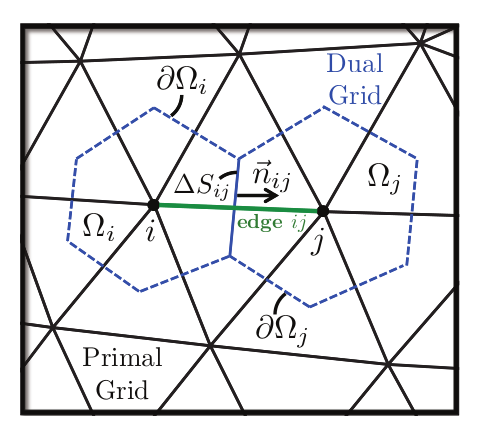
\includegraphics[width=0.5\linewidth]{figures/DualMeshControlVolume.png}
    \caption{Dual mesh control volumes surrounding two nodes, $i$ and $j$, in the domain interior.}
    % \label{fig:my_label}
\end{figure}


By virtue of the functionality of geometry-relevant source, researchers do not need to implement the area calculation step and are capable to use the face area and normal vector directly.

\end{frame}

\begin{frame}{CDriver}
CDriver controls instantiating and deleting major classes, just like a housekeeper.\\
\textbf{CDriver::StartSolver} loops over all external iterations to do the following pipeline
\begin{itemize}
    \item PreprocessExtIter
    \item DynamicMeshUpdate (optional)
    \item Run (SIngle ExtIteration)
    \item Update
    \item Monitor
    \item Output
\end{itemize}
\end{frame}

\begin{frame}{CDriver::Run }
CDriver::StartSolver method runs \emph{ExtIter} times the aforementioned pipeline. For steady and unsteady simulation, the procedure is similar, \textbf{steady} solution tends to be stable in the end, while for the \textbf{unsteady} simulation every ExtIter loop means an certain period of physical time development. 
\begin{itemize}
    \item \textbf{Preprocess}\\
            iteration\_container[iZone][Inst\_0]$\longrightarrow$ Preprocess
    \item \textbf{Zone Interface}\\
            interpolator\_container[iZone][jZone]$\longrightarrow$ Set\_TransferCoeff
            Transfer\_Data(iZone, jZone)\\
    \item \textbf{Iterate}\\
            iteration\_container[iZone][Inst\_0]$\longrightarrow$ Iterate
    \item \textbf{Check Convergence}
\end{itemize}
What does the \textbf{Iteration::Iterate} method do?
\end{frame}

\begin{frame}{CIteration::Iterate}
The CIteration::Iterate loops over all the solver to iterate in all equations.
\begin{itemize}
    \item \textbf{Update Global Parameters}\\
    config[val\_iZone]$\longrightarrow$ setGlobalParams
    \item \textbf{Solve the Equation}\\
    integration[val\_iZone][val\_iInst]...\\
    ...[FLOW\_SOL]$\longrightarrow$MultiGrid\_Iteration\\
    ...[TURB\_SOL]$\longrightarrow$SingleGrid\_Iteration\\
    ...[TRAN\_SOL]$\longrightarrow$SingleGrid\_Iteration\\
    ...[HEAT\_SOL]$\longrightarrow$SingleGrid\_Iteration
    \item \textbf{Mesh Update}
    \item \textbf{Output}
    
\end{itemize}
Now our focus moves from \emph{CIteration} class to \emph{CIntegration} class.
\end{frame}

\begin{frame}{CIntegration::Iteration}
Most simple case is CIntegration::SingleGrid\_Iteration.

\begin{itemize}
    \item \textbf{Preprocessing}
    solver\_container[iZone][iInst][FinestMesh][SolContainer\_Position]\\$\longrightarrow$ Preprocessing\\$\longrightarrow$ Set\_OldSolution \\$\longrightarrow$ Set\_Timestep
    \item \textbf{Space Integration}
    Space\_Integration(...)
    \item \textbf{Time Integration}
    Time\_Integration(...)
    \item \textbf{Postprocessing}
\end{itemize}

The space integration will invoke \textbf{CSolver} class to compute the residual.
\end{frame}

\begin{frame}
\frametitle{CSolver}
One physical problem may consist of various equations.
CSolver controls its own conservative equation. 

e.g., RANS model in SU2 has three solvers working together, FLOW\_SOL, TURB\_SOL, TRAN\_SOL.



Let's have heat equation as an example.
Different spatial residual terms coexist in one equation.
\begin{itemize}
    \item \emph{CONV}, Convective terms caused by fluid motion.
    \item \emph{VISC}, Viscous terms caused by the gradient of temperature. 
\end{itemize}

\textbf{Space\_Integration}
solver\_container[MainSolver]...\\
\textbf{CONV\_TERM}$\longrightarrow$Centered\_Residual\quad$\longrightarrow$Upwind\_Residual\\
\textbf{VISC\_TERM}$\longrightarrow$Viscous\_Residual\\
\textbf{Source\_TERM}$\longrightarrow$Source\_Residual\\
\textbf{BC}$\longrightarrow$BC\_Euler\_wall(...)...\\
\textbf{Dual\_Time}$\longrightarrow$SetResidual\_DualTime

\end{frame}


\begin{frame}{CHeatSolver VISC TERM}
Apparently, the viscous term in heat equation means the temperature tends to be the same all over the domain.

For simple situation in solid material, the heat equation reads as
\begin{equation}
    \frac{\partial T}{\partial t} - \nabla\cdot(\alpha \nabla T) =0,
\end{equation}
where $\alpha$ is the thermal diffusivity and depends on whether the material is liquid or solid.

\begin{equation}
F_{ij}=\alpha \vec{S}\cdot \nabla T=\alpha \vec{S}\cdot \frac{T_j-T_I}{\left \| d_{ij} \right \|^2}\vec{d_{ij}}
\end{equation}
\begin{equation}
    \frac{\partial F_{ij}}{\partial T_i}=-\alpha \frac{\vec{S}\cdot \vec{d_{ij}}}{\left \| d_{ij} \right \|^2}
\end{equation}
BCs are similar, contributing residuals and Jacobian matrix to the overall LARGE SPARSE matrix.
\end{frame}


\lstset{keywordstyle=\color{red},keywords={court}}
\begin{lstlisting}
  eddy_viscosity_i = 0.0;
  eddy_viscosity_j = 0.0;
  laminar_viscosity = config->GetMu_ConstantND();
  Prandtl_Lam = config->GetPrandtl_Lam();
  Prandtl_Turb = config->GetPrandtl_Turb();

  for (iEdge = 0; iEdge < geometry->GetnEdge(); iEdge++) {

    iPoint = geometry->edge[iEdge]->GetNode(0);
    jPoint = geometry->edge[iEdge]->GetNode(1);

    /*--- Points coordinates, and normal vector ---*/

    numerics->SetCoord(geometry->node[iPoint]->GetCoord(),
                       geometry->node[jPoint]->GetCoord());
    numerics->SetNormal(geometry->edge[iEdge]->GetNormal());

    Temp_i_Grad = node[iPoint]->GetGradient();
    Temp_j_Grad = node[jPoint]->GetGradient();
    numerics->SetConsVarGradient(Temp_i_Grad, Temp_j_Grad);

    /*--- Primitive variables w/o reconstruction ---*/
    Temp_i = node[iPoint]->GetSolution(0);
    Temp_j = node[jPoint]->GetSolution(0);
    numerics->SetTemperature(Temp_i, Temp_j);

    /*--- Eddy viscosity to compute thermal conductivity ---*/
    if (flow) {
      if (turb) {
        eddy_viscosity_i = solver_container[TURB_SOL]->node[iPoint]->GetmuT();
        eddy_viscosity_j = solver_container[TURB_SOL]->node[jPoint]->GetmuT();
      }
      thermal_diffusivity_i = (laminar_viscosity/Prandtl_Lam) + (eddy_viscosity_i/Prandtl_Turb);
      thermal_diffusivity_j = (laminar_viscosity/Prandtl_Lam) + (eddy_viscosity_j/Prandtl_Turb);
    }
    else {
      thermal_diffusivity_i = config->GetThermalDiffusivity_Solid();
      thermal_diffusivity_j = config->GetThermalDiffusivity_Solid();
    }

    numerics->SetThermalDiffusivity(thermal_diffusivity_i,thermal_diffusivity_j);

    /*--- Compute residual, and Jacobians ---*/

    numerics->ComputeResidual(Residual, Jacobian_i, Jacobian_j, config);

    /*--- Add and subtract residual, and update Jacobians ---*/

    LinSysRes.SubtractBlock(iPoint, Residual);
    LinSysRes.AddBlock(jPoint, Residual);

    Jacobian.SubtractBlock(iPoint, iPoint, Jacobian_i);
    Jacobian.SubtractBlock(iPoint, jPoint, Jacobian_j);
    Jacobian.AddBlock(jPoint, iPoint, Jacobian_i);
    Jacobian.AddBlock(jPoint, jPoint, Jacobian_j);
\end{lstlisting}



% \section{Physics of SU2}

\begin{frame}{Conservative Equations}
\begin{equation}
\frac{\partial \boldsymbol{U}}{\partial t}+\nabla \cdot \boldsymbol{F}^{c}-\nabla \cdot\left(\mu^{v k} \boldsymbol{F}^{v k}\right)=\boldsymbol{Q} \quad \text { in }\Omega,  \quad t>0
\end{equation}
    
\end{frame}

\subsection{Fluid Model}
\begin{frame}[allowframebreaks]
\frametitle{Reynolds-Averaged Navier–Stokes Equations (RANS)}
\begin{equation}
\left\{\begin{array}{ll}{\mathcal{R}(U)=\frac{\partial U}{\partial t}+\nabla \cdot \boldsymbol{F}^{c}-\nabla \cdot\left(\mu^{v k} \boldsymbol{F}^{v k}\right)-\boldsymbol{Q}=0} & {\text { in } \Omega, \quad t>0} \\ {v=\mathbf{0}} & {\text { on }S,} \\ {\partial_{n} T=0} & {\text { on } S} \\ {(\boldsymbol{W})_{+}=W_{\infty}} & {\text { on } \Gamma_{\infty}}\end{array}\right.
\end{equation}


\begin{equation*}
\frac{\partial \boldsymbol{U}}{\partial t}+\nabla \cdot \boldsymbol{F}^{c}-\nabla \cdot\left(\mu^{v k} \boldsymbol{F}^{v k}\right)=Q \quad \text { in } \Omega, t>0
\end{equation*}

\framebreak

\begin{equation*}
\boldsymbol{U}=\left\{\begin{array}{c}{\rho } \\ {\rho \boldsymbol{v} } \\ {\rho E}\end{array}\right\},\quad
\boldsymbol{F}^{c}=\left\{\begin{array}{c}{\rho \boldsymbol{v}} \\ {\rho \boldsymbol{v} \otimes \boldsymbol{v}+ p\mathcal{I} } \\ {\rho E \boldsymbol{v}+p \boldsymbol{v}}\end{array}\right\}
\end{equation*}

\begin{equation*}
\boldsymbol{F}^{v1}=\left\{\begin{array}{c}{\cdot} \\ {\mathcal{\tau}} \\ {\mathcal{\tau} \cdot \boldsymbol{v}}\end{array}\right\},\quad
\boldsymbol{F}^{v2}=\left\{\begin{array}{c}{\cdot} \\ {\cdot} \\ {c_p \nabla T}\end{array}\right\},\quad
Q=\left\{\begin{array}{c}{q_\rho} \\ {\boldsymbol{q}_{\rho\boldsymbol{v}}} \\ {q_{\rho E}}\end{array}\right\}
\end{equation*}

\begin{equation}
\mathcal{\tau}=\nabla \boldsymbol{v}+\nabla \boldsymbol{v}^{T}-\frac{2}{3} \mathcal{I}(\nabla \cdot \boldsymbol{v})
\end{equation}

For \textbf{ideal gas},
\begin{equation}
    p=(\gamma-1)\rho[E-\frac{1}{2}(\boldsymbol{v}\cdot \boldsymbol{v})],
\end{equation}
\begin{equation}
    T=p/(\rho R), 
\end{equation}
\begin{equation}
    c_p = \gamma R/(\gamma-1)
\end{equation}

The total viscosity is divided into a laminar $\mu_{dyn}$  and a
turbulent $\mu_{tur}$ component.
\begin{equation}
\mu^{v 1}=\mu_{\mathrm{dyn}}+\mu_{\mathrm{tur}}, \quad \mu^{v 2}=\frac{\mu_{\mathrm{dyn}}}{P r_{d}}+\frac{\mu_{\mathrm{tur}}}{P r_{t}},
\end{equation}
where $Pr_d$ and $Pr_t$ are the dynamic and turbulent Prandtl numbers,
respectively.



\framebreak
\textbf{Supported Boundary Conditions}
\begin{itemize}
    \item Euler (flow tangency) and symmetry wall,
    \item no-slip wall (adiabatic and isothermal),
    \item far-field and near-field
boundaries,
    \item characteristic-based inlet boundaries (stagnation, mass
flow, or supersonic conditions prescribed),
    \item characteristic-based
outlet boundaries (back pressure prescribed),
    \item periodic boundaries,
    \item nacelle inflow boundaries (fan face Mach number prescribed),
    \item nacelle exhaust boundaries (total nozzle temp and total nozzle
pressure prescribed).
\end{itemize}

The turbulent viscosity $\mu_{tur}$ is obtained from a suitable turbulence
model involving the flow state and a set of new variables. The (1) \textbf{Menter
shear-stress transport} model and the (2) \textbf{Spalart–Allmaras} model are two
of the most common and widely used turbulence models for the
analysis and design of engineering applications in turbulent flows.
    

\end{frame}

\begin{frame}{SU2 Framework}
\uncover<+->{\begin{equation*}
\frac{\partial U}{\partial t}+\nabla \cdot \boldsymbol{F}^{c}-\nabla \cdot\left(\mu^{v k} \boldsymbol{F}^{v k}\right)=Q \quad \text { in } \Omega, t>0
\end{equation*}
}
\uncover<+->{\[ \Downarrow \]
\begin{align*}
    \int_{\Omega_{i}} \frac{\partial U}{\partial t} d \Omega & + \sum_{j \in \mathcal{N}(i)}\left(\tilde{F}_{i j}^{c}+\tilde{F}_{i j}^{v k}\right) \Delta S_{i j}-Q\left|\Omega_{i}\right| \\ 
=\int_{\Omega_{i}} \frac{\partial U}{\partial t} d \Omega & +  R_{i}(U)=0
\end{align*}
}

For each variable in each cell, there is a residual.
\end{frame}

\begin{frame}{Two-Temperature Model for High-Speed Non-Equilibrium Flow}
    
\end{frame}

\begin{frame}{Heat Equation}
    
\end{frame}

\begin{frame}{Wave Equation}
    
\end{frame}

\begin{frame}{Poisson Equation}
    
\end{frame}

\begin{frame}{Equations of Linear Elasticity}
    
\end{frame}
\section{What's Done and Left?}

\begin{frame}{Tasks}

DONE:
\begin{itemize}
    \item $\CheckedBox$  CMaxwellVariable class
    \item $\CheckedBox$  CMaxwellSolver class except for the BC part
    
    \begin{itemize}
        \item Solver Initialization: Initial variable state setting is quite easy compared to other solver's variables. Setting to zero initially is enough.
        
        \item Spatial Residual: flux-splitting method is categorized to be the source term, while the current density influence on $dE/dt$ is will also be added.
    \end{itemize}
    
    \item $\CheckedBox$  CNumerics class using flux-splitting method to compute residual
    \item $\CheckedBox$  CDriver class
    \item $\CheckedBox$  CIntegration class
\end{itemize}

\end{frame}

\begin{frame}{Tasks}
TODO:
\begin{itemize}
    \item $\Box$  BC part of the Solver class
    \begin{itemize}
        \item Non-reflection condition.
        \item PMR, perfect matched layer.
        \item Planar EM wave as source.
        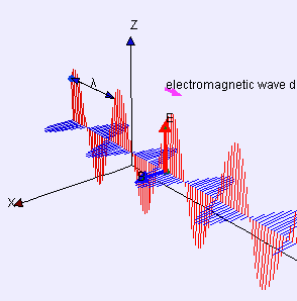
\includegraphics[width=0.2\linewidth]{figures/PlanarWave.png}
        \item Dielectric material, perfect conductor and perfect magnetized material.
    \end{itemize}
    \item $\Box$ Output function 
    \item $\Box$ Classical Test Scene Result Verification
    \item $\Box$ Thin-Wire model
    
    No similar concepts found in fluid dynamics.
\end{itemize}


\end{frame}


% \begin{frame}{Tasks}
% For the EM Maxwell module in unstructured mesh,
% \begin{itemize}
%     \item \emph{What's done?}
%     \begin{itemize}
%         \item Researched on the current stability analysis of the Maxwell flux instability.
%         \item Implemented the flux-splitting numerical method in SU2.
%     \end{itemize}
%     \item \emph{What's left?} 
%     \begin{itemize}
%         \item To implement the boundary condition flux computation.
%         \item To simulate the thin-witr model, which can be used to simulate the coil in tokamaks.
%         \item To couple different modules together.
%     \end{itemize}
% \end{itemize}


% For the magnetic reconnection simulation,
% \begin{itemize}
%     \item Maxwell module
%     \item Pressure module
%     \item Torus geometry setting
% \end{itemize}
% \end{frame}


% \section{Summer Experience}


\begin{frame}{Conferences and Reports}
 Prof. Na, as the chairman of the Integrated Operation Scenario (IOS) Group (part of ITPA), presented a report about the nonlinear MHD effect on disruption predicted by JOREK code and RNN. 
\begin{figure}
\begin{minipage}[t]{0.5\linewidth}
\centering
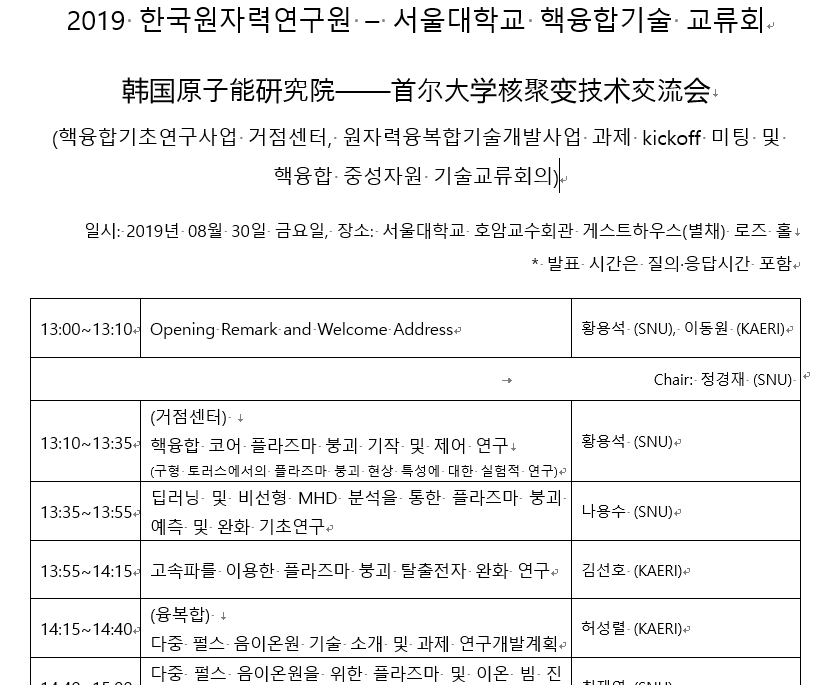
\includegraphics[width=\linewidth]{figures/ConferenceSchedule.png}
\caption{Part of Conference Schedule}
% \label{fig:side:a}
\end{minipage}%
\begin{minipage}[t]{0.5\linewidth}
\centering
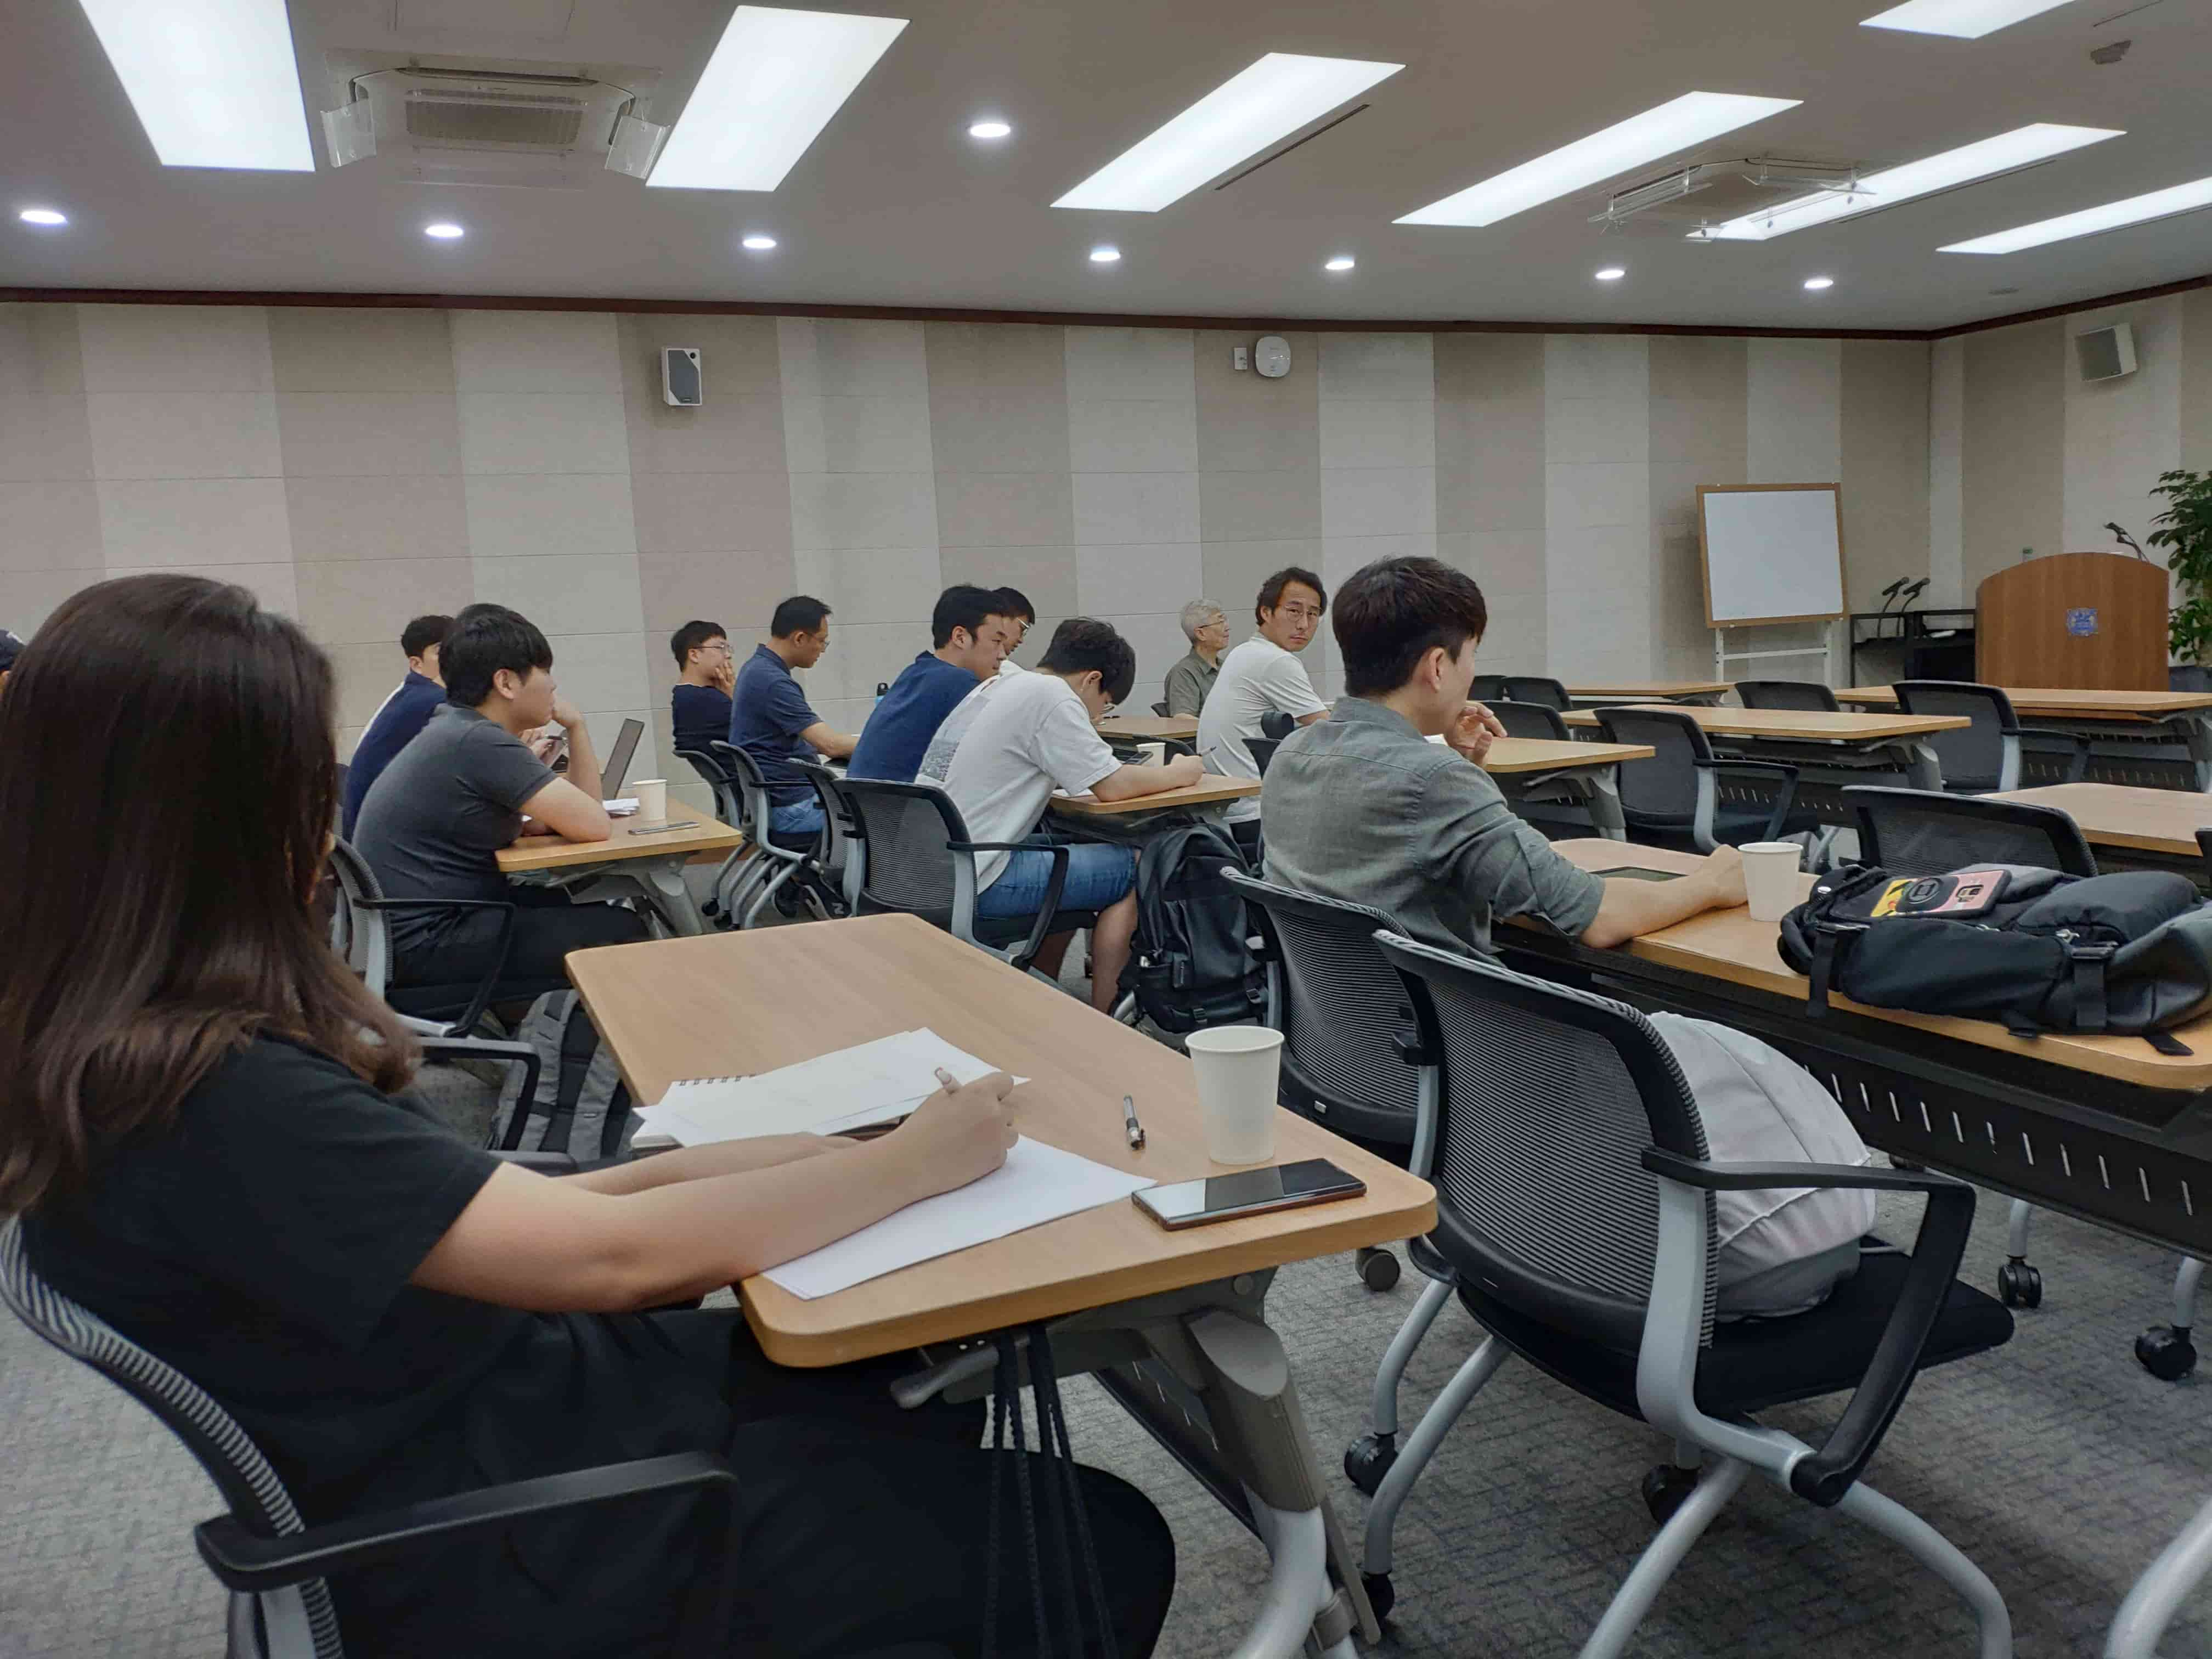
\includegraphics[width=\linewidth]{figures/conference_photo.jpg}
\caption{Conference Scene}
% \label{fig:side:b}
\end{minipage}
\end{figure}

\end{frame}

\begin{frame}{Last Weekend Hiking}
My last weekend in Seoul, our lab has a hiking to an island near Seoul.
\begin{figure}
\centering
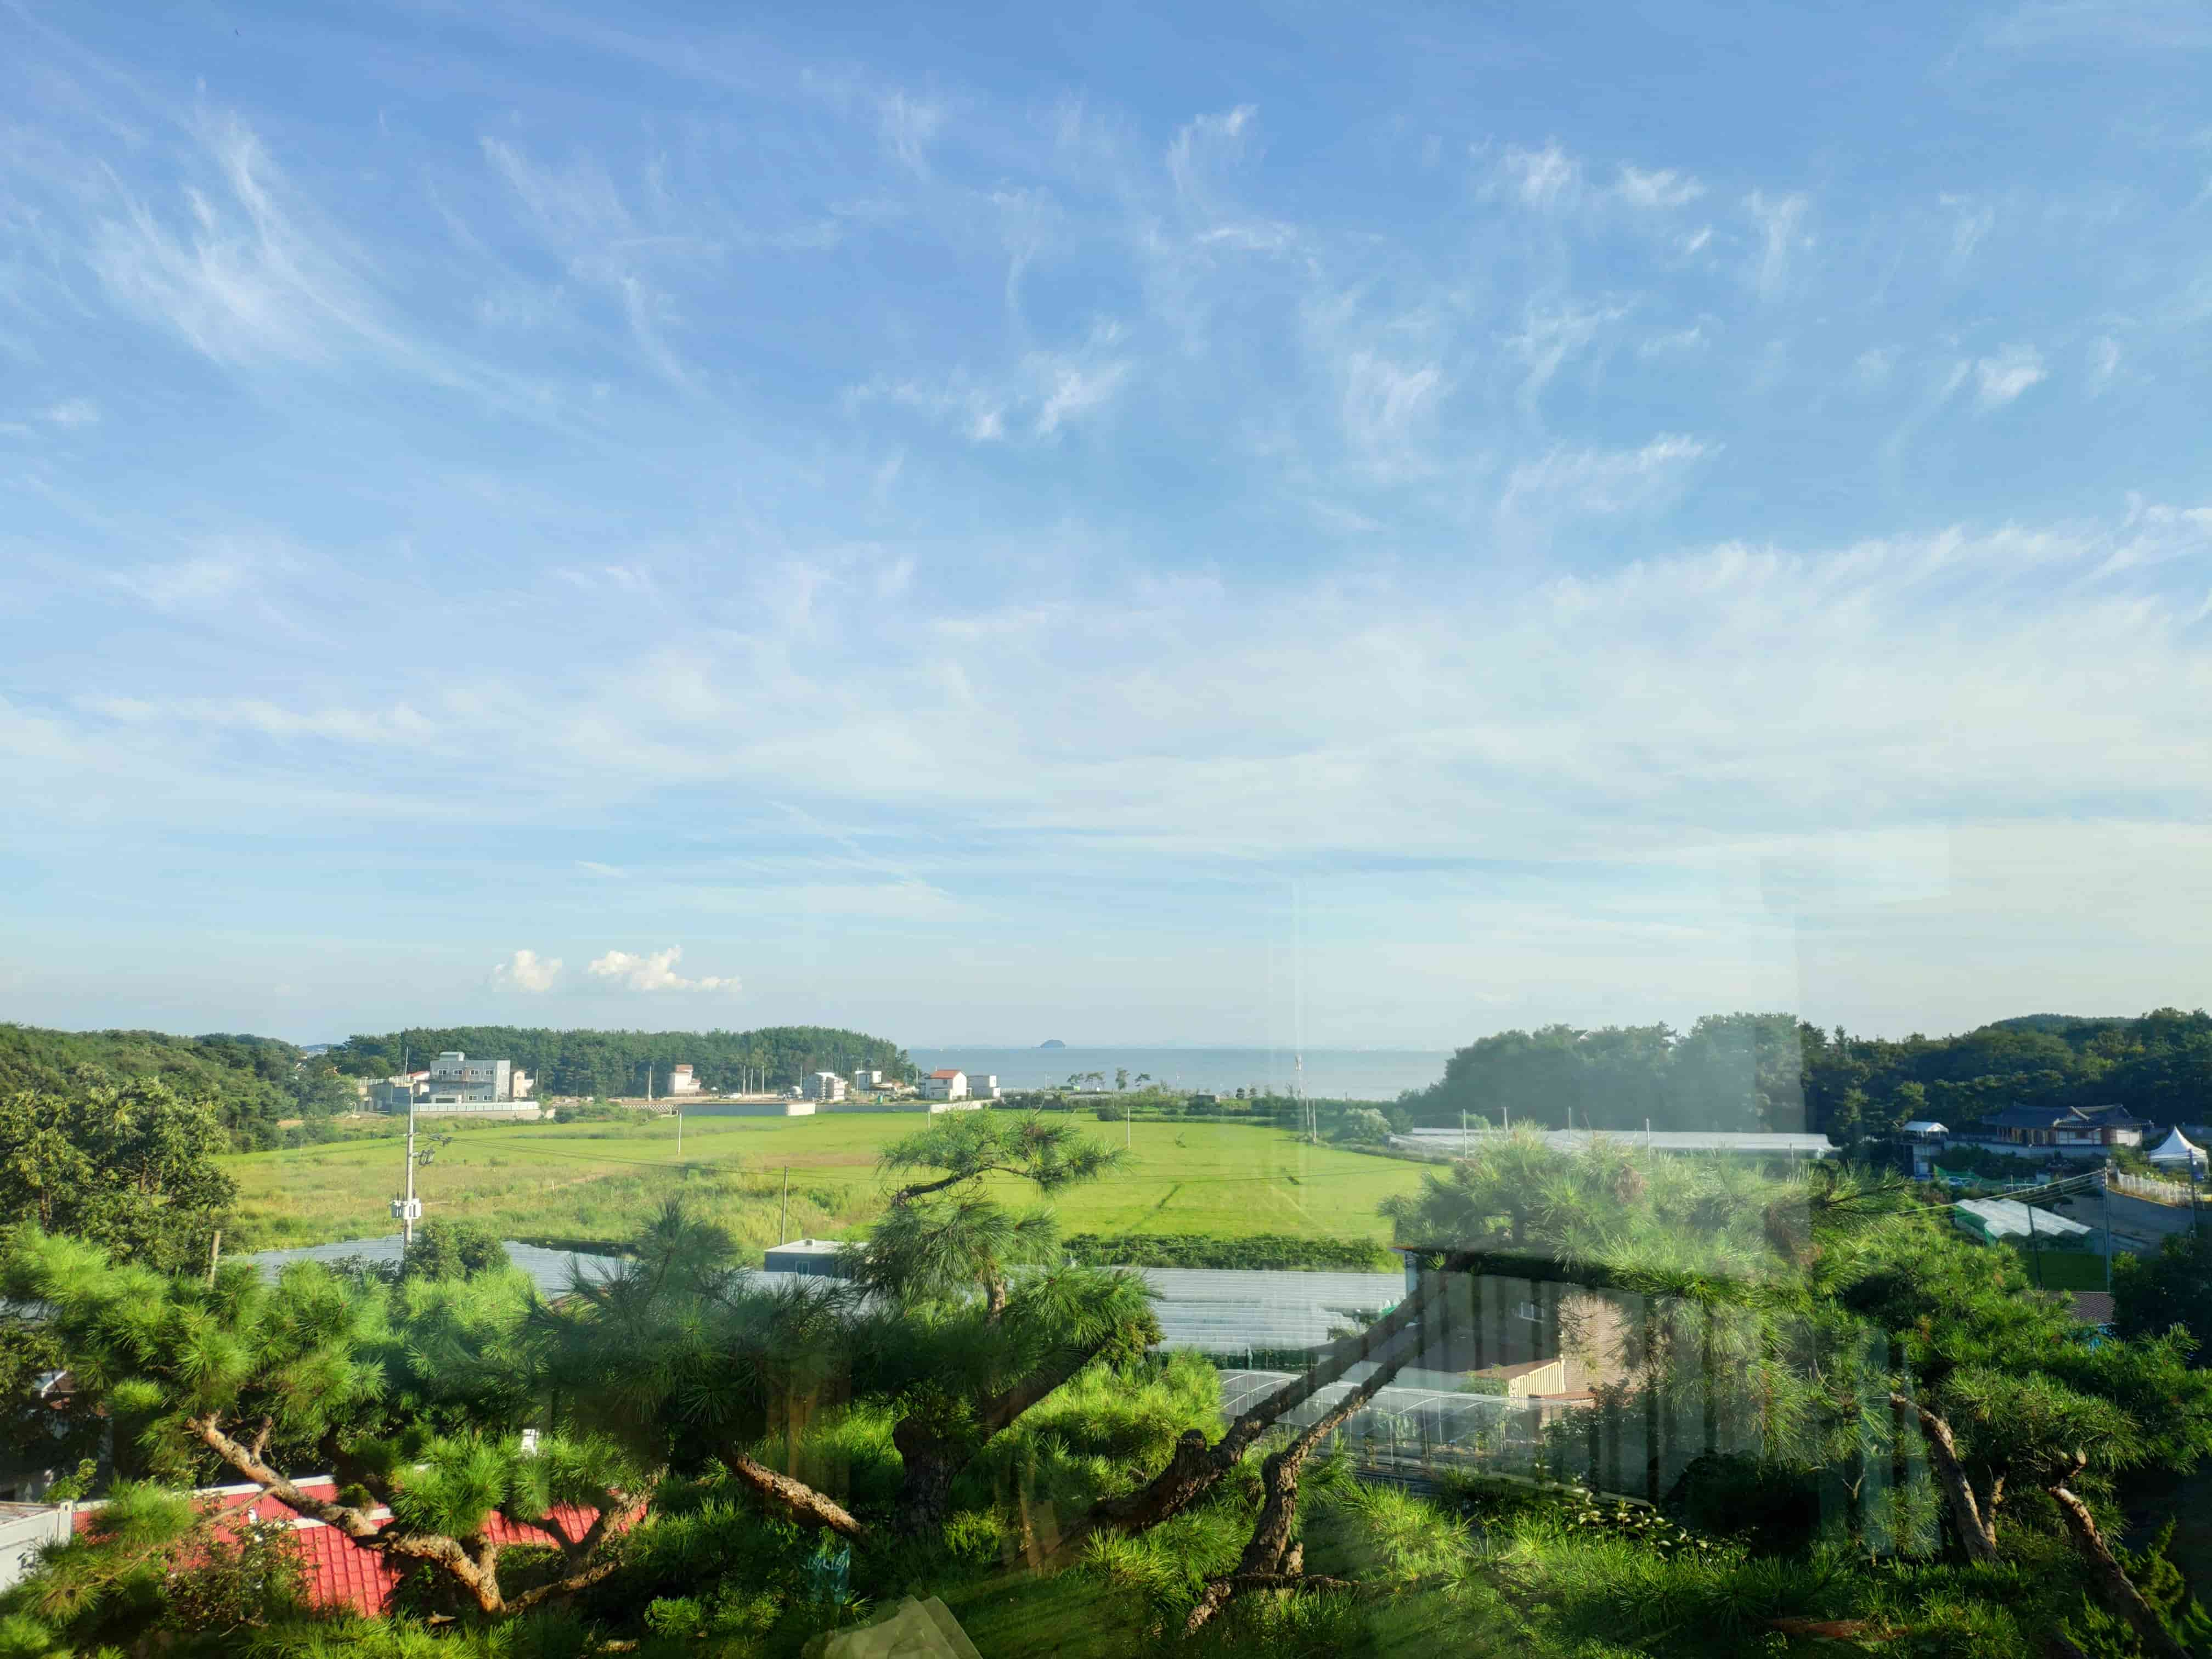
\includegraphics[width=0.9\linewidth]{figures/hiking_sight.jpg}
\end{figure}
\end{frame}

\begin{frame}{Last Weekend Hiking}

\begin{figure}
\centering
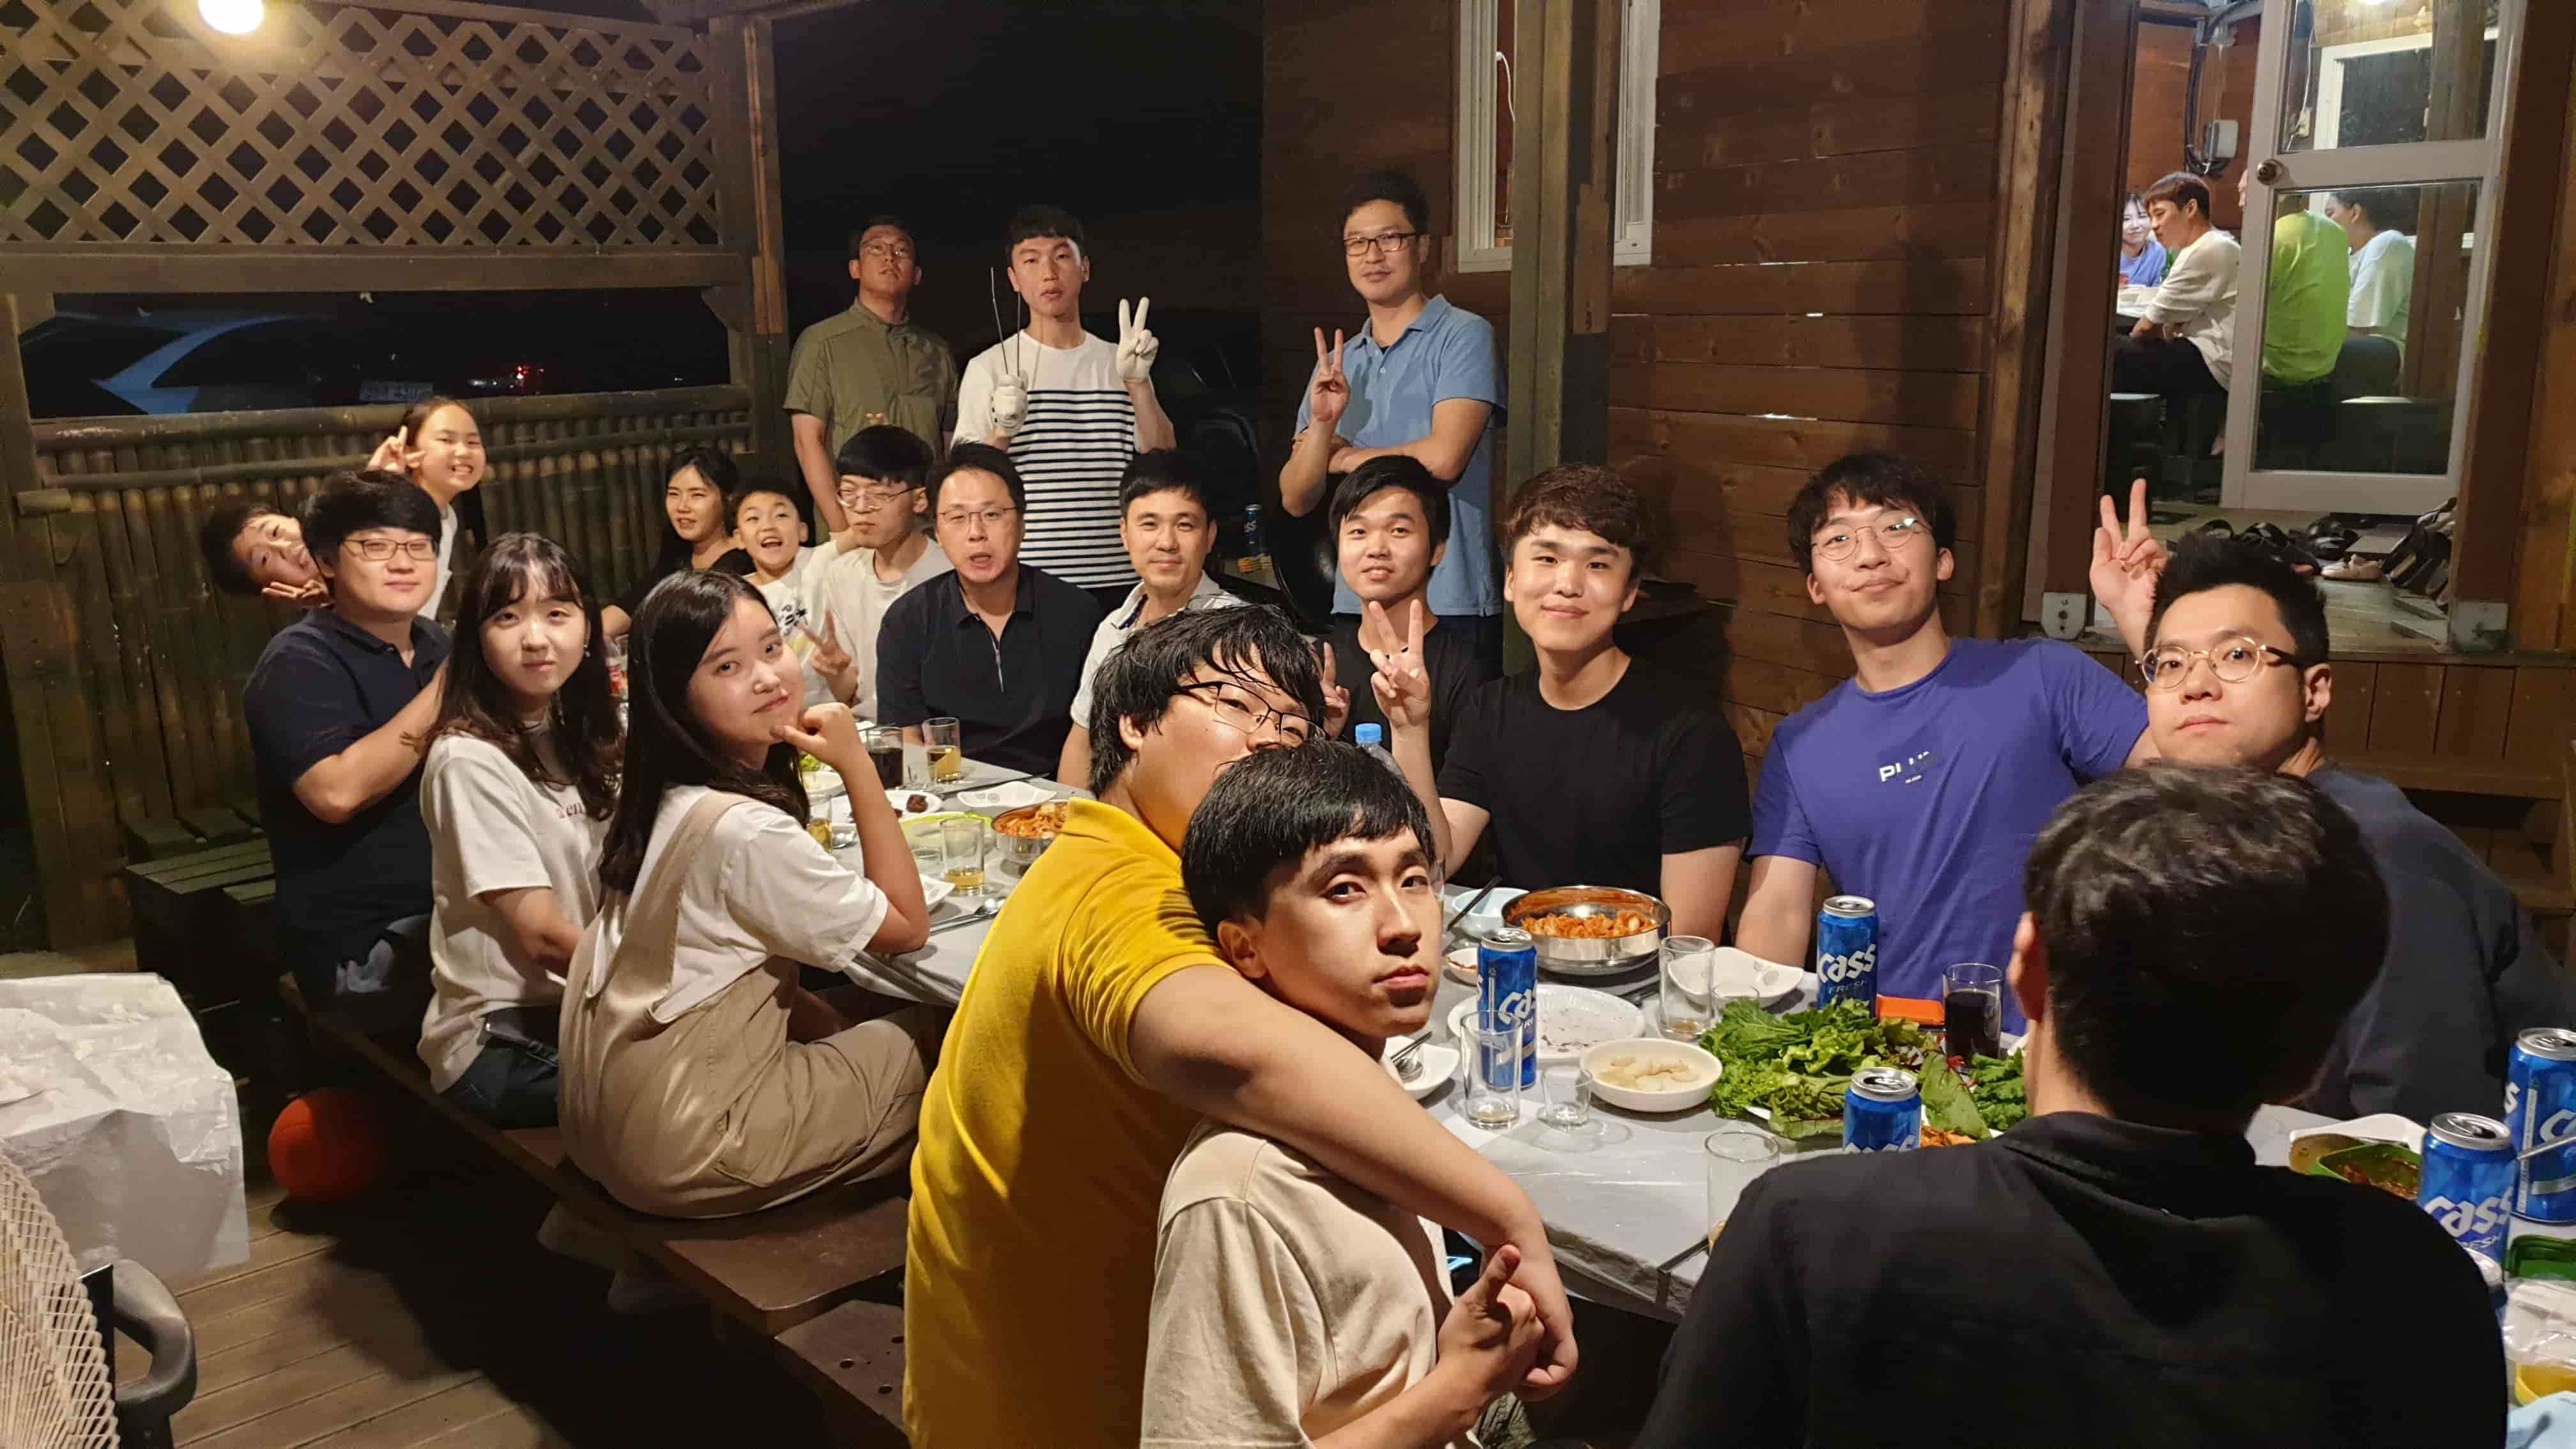
\includegraphics[width=0.9\linewidth]{figures/group_photo.jpg}
\end{figure}
\end{frame}






% %!TEX root = Intro-NLP-seminar.tex
\section{Example Applications of NLP}

\begin{frame}
\frametitle{Machine Translation (MT)}
\framesubtitle{e.g.~Google Translate}
\begin{itemize}
\item Automatic translation of a text from a \emph{source language} to a \emph{target language} by a computer, preserving the meaning
\item Some language pairs have good outputs; some not so good
\item \alert{(Why?)}
\framebreak
\item Analyse input $\longrightarrow$ processing $\longrightarrow$ Synthesise output
\item Need to ensure meaning is translated correctly
\item Need to ensure output is grammatically correct
\item \alert{`Translating' by dictionary look up or just translating words individually is \emph{not} MT}
\end{itemize}
\end{frame}

\plain{However\ldots}

\begin{frame}[allowframebreaks]
\frametitle{Use cases of MT}
\framesubtitle{What do you need MT for?}
\textcite[ch.~10]{Somers:2003} pointed out 3 use cases of MT.
\begin{itemize}
\item \textbf{Disemmination}
	\begin{itemize}
	\item Translation output to be distributed for human as-is without changes
	\item End users will have high expectations!
	\item Output must be more or less perfect and well-formed
	\item Hard -- except for language pairs with huge amount of training data
\framebreak
	\item Example Russian--English translation, suitable for dissemination:
		\begin{description}
		\item[Russian:] 18 февраля 2015 года Аналитическое управление аппарата Совета Федерации совместно с экономическим факультетом МГУ проводят научный семинар «Реалистическое моделирование».
		\item[English:] February 18, 2015 Analytical Department of the Federation Council in conjunction with the Faculty of Economics of Moscow State University conducted a scientific seminar ``The realistic simulation.''
		\end{description}
\framebreak
\item \textbf{Assimilation} 
	\begin{itemize}
	\item Just to get a rough idea of the content
	\item Output need not be perfect
	\item But choice of words should reflect original meaning
	% \item Example:
	% 	\begin{description}
	% 	\item[Iban:] Udah ujan nya ngetu terbubuh, matahari enggau emperaja lalu ayan ba langit
	% 	\item[English:] rain cease, sun and rainbow visible sky. 
	% 	\end{description}
	 \end{itemize}
\framebreak
	\item Example Japanese--English translation, for assimilation:
		\begin{description}
		\item[Japanese:] 世界中の優秀な頭脳を魅了し、研究に集中できるようなサポート体制の整った環境とはどのようなものでしょうか。
		\item[English:] Attracts the brightest minds in the world, what What are the well-equipped environment support system, such as can concentrate on research.
		\end{description}
	\end{itemize}
\framebreak
\item \textbf{Interchange}
	\begin{itemize}
	\item Translation in one-to-one communication (telephone or written correspondence).
	\item Internet: tweets, blog posts, forums
	\item Human translation is out of the question (too slow)!
	\item \emph{Any} output (even if poor) is better than \emph{no} output
%	\item Usually for shorter phrases and values
%	\item Context is still important to choose correct words to reflect similar meaning!
	\end{itemize}
\end{itemize}
\end{frame}

\begin{frame}
\frametitle{Some definitions}
\begin{description}[Source language]
\item[Utterance] An uninterrupted chain of spoken or written language
\item[Source language] The original language of an utterance
\item[Target language] The language the utterance to be translated to
\item[Language pair] a SL--TL pair for an MT process, in that direction
\end{description}

\end{frame}

%\againframe{MachineTranslation}

%\begin{frame}
%\frametitle{Automatic Summarisation}
%
%\end{frame}


\begin{frame}
\frametitle{Text and Corpus Processing}
    
\begin{itemize}[<+->]
\item Given a text or a corpus (a collection of documents)
\item Identify the most frequently occurring words; most significant words; group of words \ldots
\item Most frequently occuring: the, a, an\ldots probably not so important!
\item Most significant collocations ($n$-grams): finance, investment capital, tax returns\ldots\\
		$\longrightarrow$ document is probably about \textbf{Finance} or \textbf{Economy}
\item Useful for domain identification; document indexing for retrieval (search engine)
\end{itemize}

\end{frame}

\begin{frame}
\frametitle{Information Extraction (IE)} 

\begin{itemize}[<+->]
\item Extract ``interesting'' facts to store in a knowledge base 
\item `John stays in London. He works there for Polar Bear Design.'
	\begin{exampleblock}{Knowledge Base}
	$\text{John}_\text{PER} \xrightarrow{\text{live-in}} \text{London}_\text{LOC}$\\
	$\text{John}_\text{PER} \xrightarrow{\text{employee-of}} \text{Polar Bear Design}_\text{ORG}$
	\end{exampleblock}
\end{itemize}
\end{frame}


\begin{frame}
\frametitle{Another IE Example (Easier?)}
    
\begin{figure}
\centering
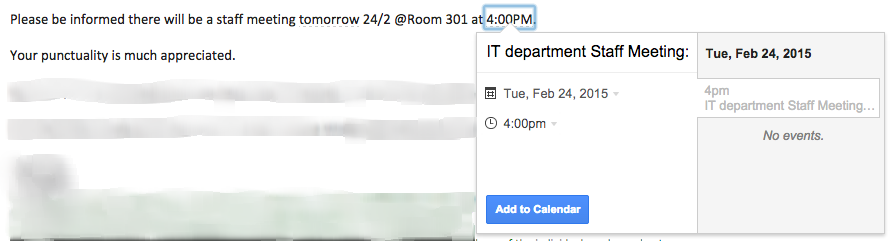
\includegraphics[width=\textwidth]{IE-event}
\end{figure}

NLP applications are often easier to design and implement with a specific use case scenario in mind

\end{frame}


\begin{frame}
\frametitle{Named Entity Recognition (NER)}

\begin{itemize}
\item Identification of proper nouns in the text
\item And classify them into catogeries of interest
\pause
\item (Typically Person, Location, Organisation, Date, Currency\ldots)
\pause
\item `\textbf{John}$_\text{PER}$ stays in \textbf{London}$_\text{LOC}$. He works there for \textbf{Polar Bear Design}$_\text{ORG}$.'
\end{itemize}

\end{frame}


\begin{frame}
\frametitle{Co-reference Resolution}

\begin{itemize}[<+->]
\item Tracking references to NEs
\item 
\tikz[baseline,remember picture]\node[anchor=base,inner sep=0pt] (john) {John}; 
stays in \tikz[baseline,remember picture]\node[anchor=base,inner sep=0pt] (london) {London};. 
\tikz[baseline,remember picture]\node[anchor=base,inner sep=0pt] (he) {He}; 
works \tikz[baseline,remember picture]\node[anchor=base,inner sep=0pt] (there) {there}; 
for Polar Bear Design. 
\tikz[overlay,remember picture]\path(he.south) edge[bend left,->,draw, >=latex'] (john.south) (there.north) edge[bend right,->,draw, >=latex'] (london.north);
\end{itemize}

\end{frame}


\begin{frame}
\frametitle{Question Answering (QA)}
\framesubtitle{e.g.~Siri}

\begin{itemize}[<+->]
\item Need to compile, index, extract a knowledge base of facts (re IE)
\item Need to analyse and interpret question to identify elements
\item Need to search knowledge base
\item May need to make inferences
\item Need to present answers in a sensible manner
\end{itemize}

\begin{columns}[T]
\begin{column}{.35\linewidth}
\begin{description}[Q:]
\item[Q:] `Where is Polar Bear Design located?'
\item[A:] London
\end{description}
\end{column}

\pause

\begin{column}{.64\linewidth}
\begin{exampleblock}{Knowledge Base}
	$\text{John}_\text{PER} \xrightarrow{\text{live-in}} \text{London}_\text{LOC}$\\
	$\text{John}_\text{PER} \xrightarrow{\text{employee-of}} \text{Polar Bear Design}_\text{ORG}$\\
	\alert{$\text{Polar Bear Design}_\text{ORG} \xrightarrow{\text{based-in}} \text{London}_\text{LOC}$}
\end{exampleblock}
\end{column}
\end{columns}

\end{frame}


\begin{frame}
\frametitle{US 2012 Presidential Election Campaign}
    
\begin{itemize}
\item \citetitle{wang2012system} \parencite{wang2012system}
\item Twitter index tracks sentiment on Obama, Romney \href{http://usatoday30.usatoday.com/news/politics/story/2012-08-01/twitter-political-index/56649678/1}{\beamergotobutton{Link}}
\item How Social Media Sentiment Impacts the Presidential Campaigns \href{http://contently.com/strategist/2012/10/24/social-media-sentiment-becomes-factor-in-presidential-campaigns/}{\beamergotobutton{Link}}
\item Tracking sentiments of a speech \href{http://sentiment.dev.ber.to/}{\beamergotobutton{Link}}
\end{itemize}

\end{frame}


\begin{frame}
\frametitle{Speech Recognition $\neq$ Voice Recognition}
\begin{itemize}[<+->]
\item Speech recognition
	\begin{itemize}
	\item Given a speech sample, what was said? `Dubai' or `Good bye'?
	\item Involves language modelling (statistical model of valid sentences)
	\end{itemize}
\item Voice recognition
	\begin{itemize}
	\item Given a speech sample, determine the identity of speaker
	\item Involves signal processing, voice signatures
	\end{itemize}
\end{itemize}
\end{frame}

\begin{frame}
\frametitle{Two Approaches} 
\begin{itemize}
\item Signal processing $\longrightarrow$ identify phonemes (sound units)
\item Language modelling $\longrightarrow$ likelihood of utterance
	\begin{itemize}
	\item `It's fun to recognize speech' or
	\item `It's fun to wreck a nice beach'
	\end{itemize}
\end{itemize}
\end{frame}
% %!TEX root = Intro-NLP-seminar.tex
\section{NLP Processing Layers}

\begin{frame}
\frametitle{Linguistic Layers in NLP}

\centering

\begin{tabular}{c @{ $\Longleftrightarrow$ } c}
Morphology & word formation\\
Syntax & sentence structure, grammar\\
Semantics & meaning\\
Pragmatics & discourse, context\\[1em]
Speech & phonemes (speech units)
\end{tabular}

\end{frame}

\plain{Examples here are for English -- other languages may need different approaches}


\subsection{Morphology}

\begin{frame}
\frametitle{Morphology}
\begin{itemize}[<+->]
	\item How words are formed
		\begin{description}[Derivation:]
			\item[Inflection:] plant $\longrightarrow$ plants, planted, planting \ldots 
			\item[Derivation:] plant $\longrightarrow$ plantation, implant \ldots
		\end{description}
	\item For Malay:
		\begin{description}[Derivation:]
		\item[Inflection:] sakit $\longrightarrow$ sakitnya; pergi $\longrightarrow$ pergilah
		\item[Derivation:] sakit $\longrightarrow$ pesakit, penyakit, sakitan\ldots
		\end{description}
	\item Morphology processing: related to words
\end{itemize}
\end{frame}


\begin{frame}
\frametitle{Tokenising}

\begin{itemize}[<+->]
	\item Split input text into processable units
	\item Just by space characters\ldots?
		\begin{itemize}
			\item 
			\tikz[baseline, start chain=going right, node distance=0.5em, every node/.style={on chain, draw, text height=1.25ex, text depth=.25ex}]
			\path node{Passers-by} node{didn't} node{go} node[draw=none]{\ldots};
		\end{itemize}
	\item Just by punctuation/word boundaries\ldots?
		\begin{itemize}
			\item \tikz[baseline, start chain=going right, node distance=0.5em, every node/.style={on chain, draw, text height=1.25ex, text depth=.25ex}]
			\path node{Passers} node{-} node{by} node{didn} node{'} node{t} node{go} node[draw=none]{\ldots};
		\end{itemize}
	\item \alert{Tokenizers need to consider natural language!}
		\begin{itemize}
			\item \tikz[baseline, start chain=going right, node distance=0.5em, every node/.style={on chain, draw, text height=1.25ex, text depth=.25ex}]
			\path node{Passers-by} node{did} node{n't} node{go} node[draw=none]{\ldots};

		\end{itemize}
\end{itemize}

\end{frame}


\begin{frame}
\frametitle{Sentence Splitting}
\begin{itemize}
	\item How to identify sentence boundaries?
	\item ``That's wonderful,' he said. `Have your people call mine. Try to arrange something by 10 a.m. tomorrow.''
\end{itemize}
\end{frame}


\begin{frame}[allowframebreaks]
\frametitle{Stemming}
    
\begin{itemize}
\item \textbf{Stem:} reduced form (word stem, base or root form) or a word
\item Need not be identical to the morphological root of the word!
\item As long as related words map to the same stem
\item Usually implemented by stripping prefix/suffix

\framebreak

\item Example stemming:
	\begin{itemize}
	\item carresses $\rightarrow$ carress
	\item ponies $\rightarrow$ poni
	\item caress $\rightarrow$ caress
	\item cats $\rightarrow$ cat
	\item producer $\rightarrow$ produc
	\item produced $\rightarrow$ produc
	\item producing $\rightarrow$ produc
	\end{itemize}

\item Can have phases/sequences of rules \parencite{porter:1980,paice:1994}
\end{itemize}

\end{frame}

\begin{frame}
\frametitle{Why Stemming?}
    
\begin{itemize}[<+->]
\item Information Retrieval -- search for documents based on keywords
\item Stem all words in documents and store as index
\item Input keyword: producer $\rightarrow$ `produc'
\item Search documents whose indices contain `produc'
\item Results will include documents containing `produce', `produced', `producer' \ldots
\end{itemize}

\end{frame}


\begin{frame}[allowframebreaks]
\frametitle{Lemmatising}

\begin{itemize}
\item \textbf{Lemma:} base form of a word or term that is used as the \emph{formal dictionary entry} for the term.
\item Lemmatising can be seen as a special form of stemming
	\begin{itemize}
	\item Stemming: outputs do not need to be real words
	\item Lemmatising: outputs are genuine words used as headwords in dictionaries
	\end{itemize}
\end{itemize}

\ex
\begingl
\gla \textsmaller{Input:} banks raised rates to fight inflation//
\glb \textsmaller{Lemmas:} bank raise rates to fight inflation//
\endgl
\xe
\end{frame}


\begin{frame}
\frametitle{Stemming vs Lemmatising}
    
\begin{itemize}
\item Stemming is much faster than lemmatising
\item But lemmatising is essential for many NLP tasks
\end{itemize}

\end{frame}

\begin{frame}
\frametitle{Would lemmatising be required for these languages?}

\begin{itemize}
\item Malay
\item Chinese
\end{itemize}

\end{frame}


\begin{frame}
\frametitle{Segmentation}
\begin{itemize}[<+->]
\item Languages without word boundaries, e.g.~Chinese, Thai, Japanese, German\ldots
\item Essential for proper understanding!
\item Chinese example: {\xiheifont 有职称的和尚未有职称的}

\ex
\xiheifont
\begingl
\gla 有 职称 的 和 尚未 有 职称 的//
\glb with position ones and {not yet} with position ones//
\endgl
\xe

\ex
\xiheifont
\begingl
\gla 有 职称 的 \alert{和尚} 未有 职称 的//
\glb with position ones \alert{monks} without position ones//
\endgl
\xe

\end{itemize}

\end{frame}


\begin{frame}
\frametitle{Technological readiness}
    
\begin{itemize}
\item For English: libraries exists to perform these tasks
\item For other languages: depends -- some are still under research and development
\end{itemize}

\end{frame}

\subsection{Syntax}

\begin{frame}
\frametitle{Syntax}
\begin{itemize}
\item How words \emph{form phrases and sentences}
\item Grammatical rules and structures!
\item Syntactic processing: extract structure of phrase/sentences
\end{itemize}
\end{frame}


\begin{frame}[allowframebreaks]
\frametitle{Part-of-Speech (POS)}

\begin{itemize}[<+->]
\item A category assigned to a word based on its grammatical and semantic properties.
\item Example: noun, verb, adjective, adverb, determiner, preposition\ldots
\item Different languages may have different sets of POS e.g.~classifier (penjodoh bilangan)
%\item Open-class words (content words): nouns, verbs, adjectives, adverbs
%\item Closed-class words (function words): determiners, pronouns, conjunctions, infinitives\ldots
\end{itemize}
\end{frame}

\begin{frame}
\frametitle{POS Tagset}
\begin{itemize}
\item English: Penn Treebank (PTB) tagset is widely adopted \parencite{marcus1993building}
\item \url{https://www.ling.upenn.edu/courses/Fall_2003/ling001/penn_treebank_pos.html}
\end{itemize}
 
\begin{center}
\begin{tabular}{ll}
\toprule
Tag & Description\\
\midrule
NN & Noun, singular or mass\\
NNS & Noun, plural\\
VB & Verb, base form\\
VBD & Verb, past tense\\
VBG & Verb, gerund or present participle\\
\ldots & \ldots\\
\bottomrule
\end{tabular}
\end{center}

\end{frame}


\begin{frame}
\frametitle{POS-tagging}
    
\begin{itemize}
\item Given an utterance, assign the most likely POS tag to each word token
\item Current libraries quite stable now (for English): $\sim 96\%$ accuracy
\end{itemize}

\ex\deftagex{basic}
\begingl
\gla \textsmaller{Input:} banks raised rates to fight inflation//
\glb \textsmaller{POS-tags:} NNS VBD NNS TO VB NN//
\endgl
\xe 

\end{frame}


\begin{frame}
\frametitle{Phrase and Sentence Structure}
    
\begin{itemize}[<+->]
\item Sentences/clauses are made up of \emph{phrases} following grammar (syntax) rules
\item Some examples:
\begin{itemize}
\item Noun phrase (NP): `a bright star', `cats', `stars and moons'
\item Verb phrase (VP): `ran', `pick the ball up'
\item Clause/sentence (S): NP VP `a bright star pick the ball up'
\end{itemize}
\item (A syntactically correct sentence doesn't guarantee it makes sense!)
\end{itemize}

\end{frame}


\begin{frame}[fragile]
\frametitle{Shallow parsing (chunking)}

\begin{itemize}

\item Identify the noun phrases, verb phrases etc but do not go into the internal structure

\begin{multicols}{2}
\begin{tikzpicture}[transform shape, scale=.8]
\Tree [.S [.NP \edge[roof]; banks ] 
	[.VP \edge[roof]; {raised rates} ] 
	[.VP \edge[roof]; {to fight inflation} ]
]
\end{tikzpicture}

\pause
\begin{tikzpicture}[transform shape, scale=.8]
\Tree [.S [.NP \edge[roof]; {A bright star} ] 
	[.VP \edge[roof]; {pick the ball up} ] 
]
\end{tikzpicture}

\end{multicols}

\end{itemize}
\end{frame}

\begin{frame}[fragile]
\frametitle{Parsing (deep parsing)}

\begin{itemize}
\item Fully building the clauses and relations in a sentence
\item Syntactic parse tree:
\begin{multicols}{2}
`Banks raised rates to fight inflation'

{\small
\begin{verbatim}
(S
  (NP (NNS banks))
  (VP (VBD raised)
    (NP (NNS rates))
    (S
      (VP (TO to)
        (VP (VB fight)
          (NP (NN inflation)))))))
\end{verbatim}
}

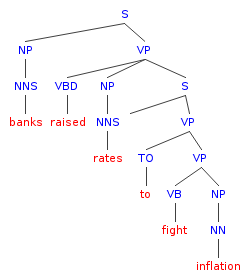
\includegraphics[width=\linewidth]{syntax-tree}

\end{multicols}
\end{itemize}
\end{frame}


\begin{frame}[fragile]
\frametitle{Dependency parsing}

\begin{itemize}
\item Find dependency relations in the text
\end{itemize}

\begin{multicols}{2}
`Banks raised rates to fight inflation'

{\small
\begin{verbatim}
nsubj(raised, banks)
root(ROOT, raised)
dobj(raised, rates)
aux(fight, to)
vmod(raised, fight)
dobj(fight, inflation)
\end{verbatim}
}

\begin{tikzpicture}[transform shape]
\Tree [.raised 
	banks
	rates
	[.fight to inflation ]
]
\end{tikzpicture}

\pause

\begin{itemize}
\item `banks' is subject of `raised'
\item `rates' is object of `raised'
\item \ldots
\end{itemize}

\end{multicols}

\end{frame}


\begin{frame}
\frametitle{Technological Readiness}
    
\begin{itemize}
\item Parsing is more difficult than POS-tagging
\item But largely solved for English
\item Varies for other languages (e.g.~OK for Chinese, no truly satisfactory one yet for Malay)
\end{itemize}

\end{frame}

\subsection{Semantic}

\begin{frame}
\frametitle{Semantic}

\begin{itemize}
\item The meaning conveyed by the text
\item Hard!
\item How to represent `meaning'?
\item Still an open question in articifial intelligence, cognitive science, psychology\ldots
\item Lots of on-going research
\end{itemize} 

\end{frame}


\begin{frame}
\frametitle{Word Sense}
    
\begin{itemize}
\item One of zero to many \emph{meanings or concepts} associated with a given \emph{head word/lemma}, as listed in a specific lexicon
\item Lexicon: a machine-readable, structured dictionary
\item May also include relations between word senses
	\begin{itemize}
	\item Synonyms, antonyms, is-a-type-of\ldots
	\end{itemize}
\end{itemize}

\end{frame}


\begin{frame}
\frametitle{Synonym Expansion}
    
\begin{itemize}
\item Example in information retrieval (search engine)
\item Search for `wizard' would also retrieve documents containing `sorcerer', `magician'
\end{itemize}

\end{frame}


\begin{frame}
\frametitle{Word Sense Disambiguation (WSD)}

\begin{itemize}
\item a.k.a.~Sense-tagging
\item Associating a word occurrence with its most likely sense, with repect to a specific lexicon
\item \textbf{Stop words:} Words that are ignored in NLP tasks, e.g.~function words in a sense-tagging task.
\end{itemize}
\end{frame}

\begin{frame}
\frametitle{How to identify stop words?}

\begin{itemize}
\item Open-class words (content words): nouns, verbs, adjectives, adverbs
\item Closed-class words (function words): determiners, pronouns, conjunctions, infinitives\ldots
\end{itemize}

\ldots so WSD needs POS-tagging and lemmatisation first

\end{frame}

\begin{frame}
\frametitle{WSD Example}

\begin{exampleblock}{Senses of bank.n in WordNet}
\begin{enumerate}
\item sloping land (especially the slope beside a body of water)
\item a financial institution that accepts deposits and channels the money into lending activities
\item a long ridge or pile
\item \ldots
\end{enumerate}
\end{exampleblock}

\ex\deftagex{basic}
\begingl
\gla \textsmaller{Input:} banks raised rates to fight inflation//
\glb \textsmaller{Sense-tags:} bank.n.2 raise.v.13 rates.n.1 {} fight.v.1 inflation.n.1//
\endgl
\xe     
\end{frame}


\begin{frame}
\frametitle{Concept Tagging}
    
\begin{itemize}
\item Label each sense in the input with a concept tag \\
(Example below uses WordNet--SUMO mapping)
\end{itemize}

\lingset{everyglb={\footnotesize}, everyglc={\scriptsize\scshape}}
\ex\deftagex{basic}
\begingl
\gla \textsmaller{Input:} banks raised rates to fight inflation//
\glb \textsmaller{Sense-tags:} bank.n.2 raise.v.13 rates.n.1 {} fight.v.1 inflation.n.1//
\glc \textsmaller{\upshape Concept tags:} Corporation Increasing Tax {}  ViolentContest Increasing//
\endgl
\xe 

\end{frame}


\begin{frame}
\frametitle{Information Extraction}

\begin{itemize}
\item Examples as given earlier
\item Named entity recognition
\item Coreference resolution
	\begin{itemize}[<+->]
	\item `The cat climbed onto the chair. It yawned and slept.'
	\item `It' = `the cat'? `the chair'?
	\item `cat' $\xrightarrow{\text{is-a}}$ \textsc{animal} $\xrightarrow{\text{is-a}}$ \textsc{animate object}
	\item `chair' $\xrightarrow{\text{is-a}}$ \textsc{furniture} $\xrightarrow{\text{is-a}}$ \textsc{inanimate object}
	\item \textsc{animate object} $\xrightarrow{\text{capable-of}}$ `yawn', `sleep'
	\item $\therefore$ `It' = `the cat'
	\end{itemize}
\end{itemize}

\end{frame}



\subsection{Pragmatics}

\begin{frame}
\frametitle{Pragmatics}

\begin{itemize}[<+->]
\item Processing text by inclduing context
\item Scenario, behavior, cultural, etc
	\begin{description}[<+->]
	\item[Q] `Can you pass me the salt?'
	\item[Machine] `Yes.'
	\item[Human] [picks up salt shaker and hands over]
	\end{description} 
	\begin{description}[<+->]
	\item[Teacher] `This is your assignment.'
	\item[Student] `What is assignment? Can eat one ah?'
	\item[Machine] `An assignment is your homework. It is not edible.'
	\item[Teacher] [rolls eyes and ignores comment]
	\end{description} 
\item `He opened the fridge.' (because he was hungry?)
\item \textbf{VERY HARD!!!}
\end{itemize}

\end{frame}


\begin{frame}
\frametitle{Speech}

\begin{itemize}[<+->]
\item Existing libraries: Android, eSpeak, Microsoft SAPI\ldots
\item Support for English is satisfactory for FYP purposes
\item (Not so good for other languages especially recognition)
\item Sounds mechanical!
\item Prosody: more natural-sounding, with emotions etc (R\&D!)
\end{itemize}
\end{frame}


% \begin{frame}
% \frametitle{Speech Synthesis: More Details}
% \begin{itemize}[<+->]
% \item Basic unit: \alert{phonemes}
% \item Speech synthesis common steps:
% 	\begin{itemize}
% 	\item Look up pronunciation coding in dictionary\\
% 		e.g.~SAMPA phonemes (MBROLA); Krishenbaum (eSpeak)\\
% 	\item `This is some phonetic text input'
% 	\item \lstinline|D,Is Iz sVm f@n'EtIk t'Ekst 'InpUt|
% 	\end{itemize}
% \end{itemize}

% \end{frame}
% %!TEX root = Intro-NLP-seminar.tex

\section{Example Individual Projects using NLP}

\begin{frame}
\frametitle{Translator Aid for Travellers}
    
\centering
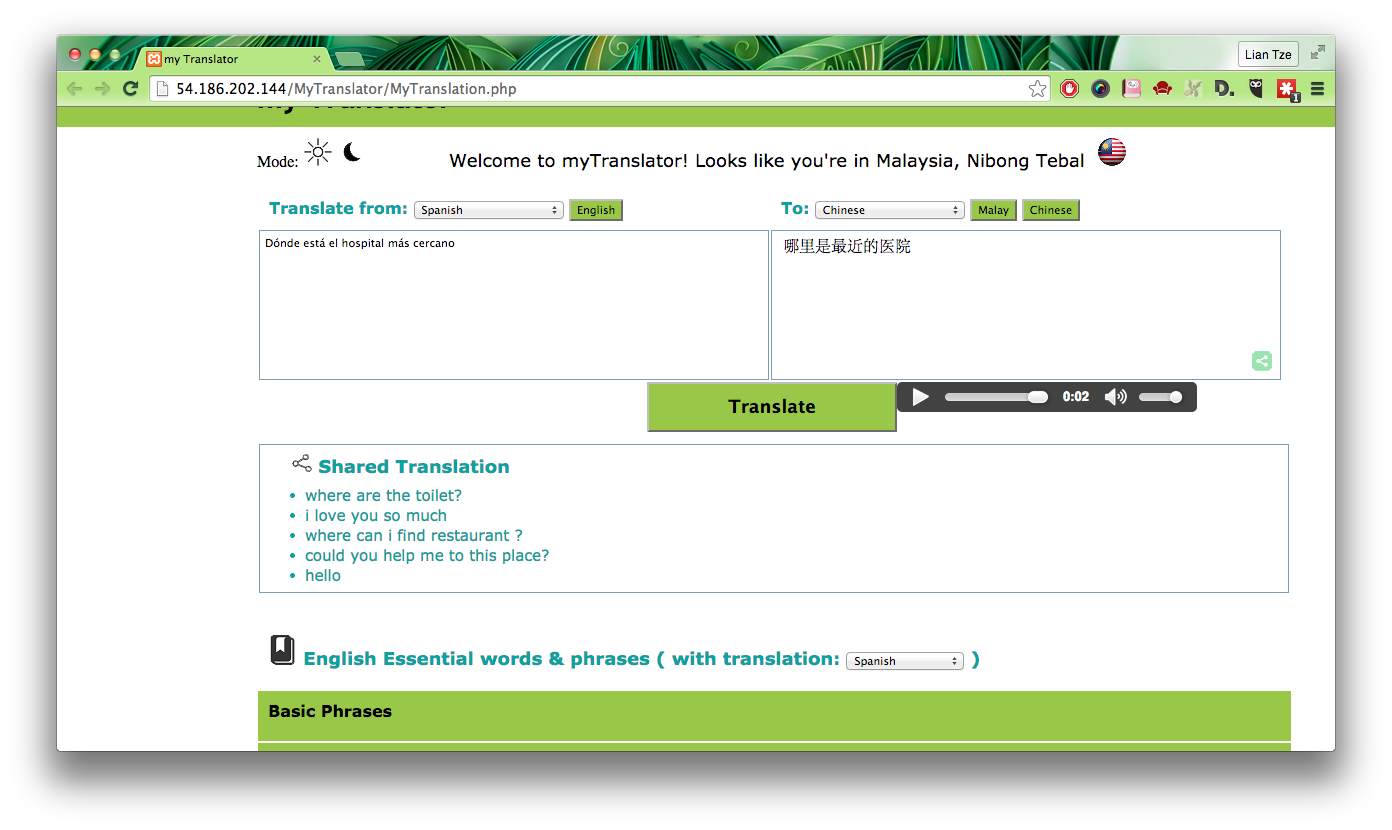
\includegraphics[width=\textwidth]{mytranslator}

\end{frame}


\begin{frame}
\frametitle{Bloom's Taxonomy Level Categorisation}
    
\centering
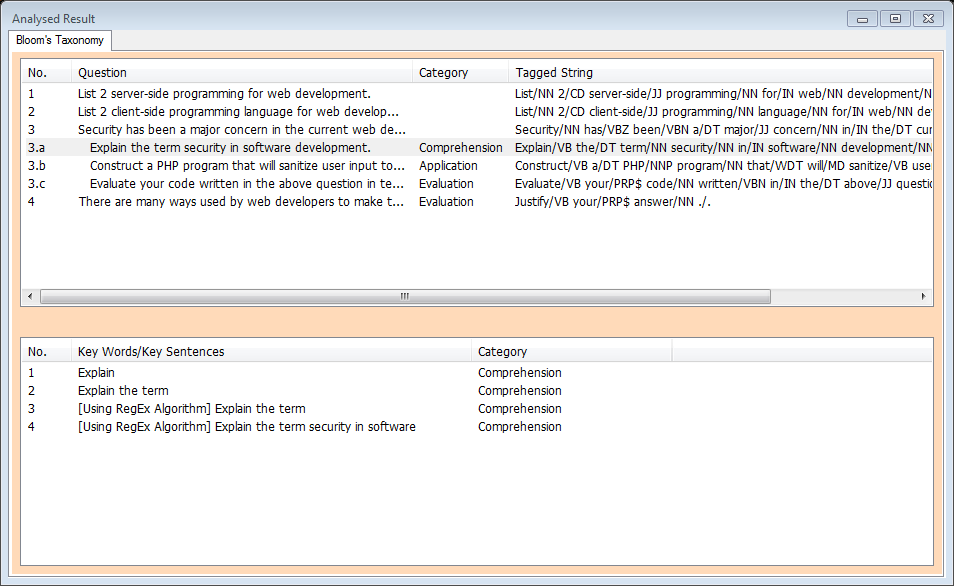
\includegraphics[width=\textwidth]{bloom-debug}

\end{frame}


\begin{frame}
\frametitle{More Examples}
    
\begin{itemize}
\item Named entity recognition including Malaysian names
\item Intelligent meaning lookup for mixed language input with spelling error detection
\item *Sentiment analysis of forum posts
\item *Information extraction to identify problem parameters
\item *Keyword extraction from paper publications
\end{itemize}
 
\end{frame}

%\begin{frame}
%\frametitle{Named Entity Recognition for Malay}
%\end{frame}


%\begin{frame}
%\frametitle{Intelligent Lookup with Mixed-language Input}
%\end{frame}

% \plain{End of Session 1\\See you next week!}

% %!TEX root = Intro-NLP-seminar.tex
\section{WordNets: lexical semantic networks}

\newcommand{\mysynset}[1]{\text{(#1)}}
\newcommand{\myrel}[1]{\text{\emph{\color{purple}#1}}}
\newcommand{\myword}[1]{\text{`#1'}}
\newcommand{\myconcept}[1]{\text{\scshape #1}}
\newcommand{\myinst}[1]{\text{\scshape\color{green!30!black} #1}}

\begin{frame}
\frametitle{WordNet: An Electronic Lexical Database}

\begin{itemize}
\item \parencite{miller:wordnet:1995}
\item Developed by Princeton University Cognitive Science Laboratory for (American) English
\item Lexical entries organised by \emph{meaning} (semantic content)
\item Wordnets for many other languages have been developed
%\item For humans: new ways of navigating a dictionary/lexicon to learn about words
%\item For computers: resource for performing (some level of) semantic analysis on natural language text
\end{itemize}
\end{frame}

\subsection{Synsets}
\begin{frame}
\frametitle{Synsets = ``synonym set''}
\begin{itemize}
\item Basic unit; represents a word meaning by \alert{synonyms}, \alert{gloss} and \alert{relations to other synsets}
\item Different senses of a word (collocation, phrasal verb, etc.) are placed in different synsets according to parts-of-speech
\item Each synset contains senses of different words that are considered synonymous
%\item For each synset:
%  \begin{itemize}
%    \item gloss
%    \item semantic field
%    \item example usage(s)
%    \item sentence frame (verbs only)
%  \end{itemize}
\end{itemize}
\end{frame}

\begin{frame}[fragile]
\frametitle{First 3 senses for noun ``court''}

\begin{itemize}
	\item 3 synsets, one for each sense (meaning)
	\item Each synset contain member lemmas with same meaning, same POS
	\item Each synset has a definition text; may have example sentence
\end{itemize}

\bigskip

\lstset{keywordstyle=\color{red},keywords={court}}
\begin{lstlisting}
<noun.group> court, tribunal, judicature - (an assembly (including one or more judges) to conduct judicial business)

<noun.group> court, royal_court - (the sovereign and his advisers who are the governing power of a state)

<noun.artifact> court - (a specially marked horizontal area within which a game is played; "players had to reserve a court in advance")
\end{lstlisting}

\end{frame}


\begin{frame}
\frametitle{Synset Organisation}
    
\begin{itemize}
\item 4 synset categories

\bigskip

\begin{center}
\begin{tabular}{l >{\ttfamily}c c}
\toprule
Category & POS code & numerical prefix\\
\midrule
noun & n & 1 \\
verb & v & 2 \\
adjective & a, s & 3 \\
adverb & r & 4 \\
\bottomrule
\end{tabular}
\end{center}

\bigskip

\item Primary key: 9-digit synset ID \alert{or} POS code + 8-digit synset ID
\item WN3.0 synset (court, tribunal, judicature) can be identified by \alert{108329453} or \alert{n-08329453} or \alert{08329453-n} in different systems
\end{itemize}
\end{frame}

\begin{frame}
\frametitle{Mapping Stanford Parser POS codes to WN POS code}

\begin{algorithmic}
\STATE \COMMENT{Ignore all other POS when looking up WN}
\IF{\texttt{\$stanfordPOS} starts with `N'}
	\STATE \texttt{\$wnPOS} $\leftarrow$ `n'
	\STATE \texttt{\$wnPOSnum} $\leftarrow$ 1

\ELSIF{\texttt{\$stanfordPOS} starts with `V'}
	\STATE \texttt{\$wnPOS} $\leftarrow$ `v'
	\STATE \texttt{\$wnPOSnum} $\leftarrow$ 2

\ELSIF{\texttt{\$stanfordPOS} starts with `J'}
	\STATE \texttt{\$wnPOS} $\leftarrow$ \{`a', `s'\}
	\STATE \texttt{\$wnPOSnum} $\leftarrow$ 3

\ELSIF{\texttt{\$stanfordPOS} starts with `R'}
	\STATE \texttt{\$wnPOS} $\leftarrow$ `r'
	\STATE \texttt{\$wnPOSnum} $\leftarrow$ 4
\ENDIF 
\end{algorithmic}


\end{frame}


\subsection{Relations}
\begin{frame}
\frametitle{Noun Synset Relations}
%\framesubtitle{Nouns}
%WordNet specifies relations between synsets and (compound) words

%\begin{exampleblock}{Noun Synset Relations}
\mode<presentation>{\small}
\begin{description}
\item[hypernymy] \mysynset{court, royal court} \myrel{is-a-kind-of} \mysynset{government, authorities, regime}
\item[holonymy] \mysynset{finger} \myrel{is-part-of} \mysynset{hand, manus, mitt, paw} \\
                \mysynset{flour} \myrel{is-substance-of} \mysynset{bread}, \mysynset{dough}, \mysynset{pastry} \\
                \mysynset{jury} \myrel{is-member-of} \mysynset{court, tribunal, judicature}
\item[instance] \mysynset{Mozart, Wolfgang Amadeus Mozart} \myrel{is-instance-of} \mysynset{composer}
\end{description}
(\ldots{}and their respective inverse relations)
%\end{exampleblock}
\end{frame}

\begin{frame}
\frametitle{Verb Synset Relations}
%\framesubtitle{Verbs}
%WordNet specifies relations between synsets and (compound) words

%\begin{exampleblock}{Verb Synset Relations}
\mode<presentation>{\small}
\begin{description}
\item[hypernymy] \mysynset{stroll, saunter} \myrel{is-one-way-to} \mysynset{walk}
\item[troponymy] \mysynset{fear} \myrel{has-specific-way} \mysynset{panic}
\item[cause] \mysynset{teach} \myrel{causes} \mysynset{learn, larn, acquire}
\item[entailment] \mysynset{buy, purchase} \myrel{entails} \mysynset{pay}, \mysynset{choose, take, select, pick out}
\item[verb frames] \mysynset{attack, assail}: \\\texttt{Somebody --s something}\\\texttt{Somebody --s somebody}\\(very simple, without any extra info)
\end{description}
%\end{exampleblock}
\end{frame}

\begin{frame}
\frametitle{Lexical Relations}
\mode<presentation>{\small}
\begin{description}
\item[antonymy] \myword{ugliness} \myrel{$\times$} \myword{beauty}, 
                \myword{pull} \myrel{$\times$} \myword{push},\\
                \myword{difficult} \myrel{$\times$} \myword{easy}, 
                \myword{quickly} \myrel{$\times$} \myword{slowly}
\item[attribute] \myword{strength} \myrel{has-attributes}: \myword{delicate}, \myword{rugged}, \myword{weak}, \myword{strong}
\item[derivation] \myword{maintain} \myrel{is-derivationally-related-to} \myword{maintainable}, \myword{maintenance}, \myword{maintainer}
\item[domain] \myword{medicine} \myrel{topic-has-terms}: \myword{acute}, \myword{fulgurating}, \myword{gauze}, \ldots\\
              \myword{France} \myrel{region-has-terms}: \myword{Battle of Valmy}, \myword{Bastille}, \myword{jeu d'esprit}, \ldots\\
              \myword{colloquialism} \myrel{usage-has-terms}: \myword{lousy}, \myword{humongous}, \myword{gobsmacked}, \ldots
\item[pertainym] \myword{biannual} \myrel{pertains-to} \myword{year}, 
                 \myword{ancestral} \myrel{pertains-to} \myword{ancestor},
                 \myword{Liverpudlian} \myrel{pertains-to} \myword{Liverpool}
\item[participle] \myrel{a} \myword{handheld} \myrel{something-participates-in} \myword{hold}
\end{description}
\end{frame}

\subsection{Getting the Data}

\begin{frame}
\frametitle{Princeton WordNet Data}
    
\begin{itemize}[<+->]
\item Browse/explore online: \url{http://wordnet.princeton.edu/}
\item Searching WordNet: APIs for many programming languages available
\item \ldots But I recommend downloading WordNet as MySQL data
\item Then use whatever programming language you like to query
\end{itemize}

\end{frame}


\begin{frame}[fragile]
\frametitle{WordNet SQL}
    
\begin{itemize}
\item \url{http://wnsql.sourceforge.net/}
\item \menu{Download > wnsql > mysql > 3.0 > mysql-3.0.0-30-wn-30.zip} Unzip. 
\item Create a MySQL database, e.g.~ \texttt{wordnet30}
\item Start a Windows command prompt.\\\menu{Windows Start > Run} type \menu{cmd} \return

\begin{lstlisting}[backgroundcolor=\color{black},basicstyle=\ttfamily\color{green}, 
escapechar=|, framexleftmargin=1em, xleftmargin=1em]
> cd <folder containing unzipped contents> |\return|
> restore.bat |\return|
\end{lstlisting}

\item You'll be prompted for the database name, username and password. Wait while the data is copied into tables.

\item (May need to add \path{C:\xampp\mysql\bin} to system path)
\end{itemize}

\end{frame}



\begin{frame}[fragile]
\frametitle{Some Tables in WN-MySQL}
    
\begin{tikzpicture}[every node/.style={rectangle split, rectangle split parts=2, draw},
every text node part/.style={align=center}] 
\node (words) [text width=4em] 
{words \nodepart{two}{\textbf{wordid}\\lemma}};

\node (senses) [text width=5em, right=3em of words]
{senses \nodepart{two}\textbf{senseid}\\wordid\\synsetid\\sensenum\\\ldots};

\node (synsets) [text width=5em, right=3em of senses]
{synsets \nodepart{two}\textbf{synsetid}\\pos\\definition\\\ldots};

\path[-crow's foot] (words) edge (senses);
\path[-crow's foot] (synsets) edge (senses);

\pause

\node (semlinks) [text width=5em, right = 4em of synsets]
{semlinks \nodepart{two}synset1id\\synset2id\\linkid};

\node (linktypes) [text width=5em, below = 3em of semlinks]
{linktypes \nodepart{two}\textbf{linkid}\\link\\\ldots};

\path[crow's foot-crow's foot] (semlinks) edge (synsets);
\path[-crow's foot] (linktypes) edge (semlinks);
\end{tikzpicture}

\end{frame}

\begin{frame}[fragile]
\frametitle{Querying Synsets (Senses) of a Lemma}
    
\begin{lstlisting}[language=SQL]
SELECT lemma, synsetid, definition
FROM words INNER JOIN senses USING (wordid)
     INNER JOIN synsets USING (synsetid)
WHERE lemma = 'plant' AND pos = 'n';
\end{lstlisting}

\begin{lstlisting}[basicstyle=\ttfamily\scriptsize,columns=fixed]
+-------+-----------+--------------------------------------------+
| lemma | synsetid  | definition                                 |
+-------+-----------+--------------------------------------------+
| plant | 100017222 | (botany) a living organism ....            |
| plant | 103956922 | buildings for carrying on industrial labor |
| plant | 105906080 | something planted secretly for...          |
| plant | 110438470 | an actor situated in the audience          |
+-------+-----------+--------------------------------------------+
4 rows in set (0.00 sec)
\end{lstlisting}

\end{frame}


\begin{frame}[fragile]
\frametitle{Querying Synonyms of a Particular Sense (Synset)}
    
\begin{lstlisting}[language=SQL]
SELECT lemma
FROM words INNER JOIN senses USING (wordid)
     INNER JOIN synsets USING (synsetid)
WHERE synsetid = 103956922;
\end{lstlisting}

\begin{lstlisting}
+------------------+
| lemma            |
+------------------+
| industrial plant |
| plant            |
| works            |
+------------------+
3 rows in set (0.00 sec)
\end{lstlisting}

\end{frame}


\begin{frame}[fragile]
\frametitle{Looking up Semantic Relations}

\begin{lstlisting}[language=SQL]
SELECT synset2id
FROM semlinks INNER JOIN synsets A 
                 ON (A.synsetid = semlinks.synset1id)
              INNER JOIN linktypes USING (linkid)
WHERE A.synsetid = 103956922 AND LINK = 'hypernym';

SELECT lemma
FROM words INNER JOIN senses USING (wordid)
     INNER JOIN synsets USING (synsetid)
WHERE synsetid = 102914991;
\end{lstlisting}

\begin{columns}[T]
\begin{column}{.45\textwidth}
\begin{lstlisting}[basicstyle=\ttfamily\footnotesize]
+-----------+
| synset2id |
+-----------+
| 102914991 |
+-----------+
1 row in set (0.00 sec)
\end{lstlisting}
\end{column}

\begin{column}{.49\textwidth}
\begin{lstlisting}[basicstyle=\ttfamily\footnotesize]
+------------------+
| lemma            |
+------------------+
| building complex |
| complex          |
+------------------+
2 rows in set (0.00 sec)
\end{lstlisting}
\end{column}
\end{columns}

\end{frame}


\subsection{Other Lexical Resources Linking to WordNet}

\begin{frame}
\frametitle{Multilingual Wordnets}
    
\begin{itemize}[<+->]
\item Wordnets in different languages -- same architecture 
\item Some free, some not: \url{http://globalwordnet.org/}
\item Almost all are `linked' to PWN (English) by \alert{synsetid}
\item WordNet Bahasa (\url{http://wn-msa.sourceforge.net/}) \parencite{Bond:etal:WordNetBahasa:2014}
\item More languages: Open Multilingual WordNet (\url{http://compling.hss.ntu.edu.sg/omw/}) \parencite{Bond:Paik:2012}
\end{itemize}

\end{frame}

\begin{frame}
\frametitle{Looking up Synsets in Other WordNets}
%\begin{itemize}
%\item Refer to relations between English WordNet synsets
%\item Copy selected relations over to Malay WordNet where possible
%\end{itemize}

%\includegraphics[width=\textwidth]{synsets-svg}
\begin{center}

\tikzstyle{synset}=[text width=15mm, font=\footnotesize,text centered]
\tikzstyle{arrlabel}=[<-,above,font=\scriptsize]
\tikzstyle{corr}=[<->,dashed]
\tikzstyle{every edge}=[draw,>=stealth']
\begin{tikzpicture}
\path[node distance=32mm] node[synset] (dictionary) {(dictionary, lexicon)}
      node[synset,right of=dictionary] (wordbook) {(wordbook)}
      edge[arrlabel] node {hyper} (dictionary)
      node[synset,right of=wordbook,text width=22mm] (reference) {(reference,\\reference book)}
      edge[arrlabel] node {hyper} (wordbook)
      node[synset,right of=reference,text width=] (book) {(book)}
      edge[arrlabel] node {hyper} (reference);

\node[above of=dictionary,xshift=45mm,yshift=10mm,font=\bfseries] {English};

\begin{scope}[font=\footnotesize\color{mLightBrown}]
\node[above of=dictionary] {106418901};
\node[above of=wordbook] {106418693};
\node[above of=reference] {106417598};
\node[above of=book] {106410904};
\end{scope}

\begin{scope}[node distance=20mm]
\uncover<2->{
\path node[synset,below of=dictionary] (kamus) {(leksikon, kamus)}
      edge[corr] (dictionary)
      node[synset,below of=reference] (rujukan) {(rujukan)}
      edge[corr] (reference)
      node[synset,below of=book,text width=] (buku) {(buku)}
      edge[corr] (book);
\node[below of=dictionary,yshift=-15mm,xshift=45mm,font=\bfseries] {Malay};
}
\uncover<3->{
\path (rujukan) edge[arrlabel] node{hyper} (kamus);
}
\uncover<4->{
\path (buku) edge[arrlabel] node{hyper} (rujukan);
}
\end{scope}

\uncover<5->{
\begin{scope}[font=\footnotesize\color{mLightBrown}]
\node[below of=kamus] {06418901-n};
\node[below of=rujukan] {06417598-n};
\node[below of=buku] {06410904-n};
\end{scope}

}
\end{tikzpicture}
\end{center}
\end{frame}

\begin{frame}
\frametitle{Other WordNet-based Resources}
    
\begin{itemize}[<+->]
\item SentiWordNet \parencite{baccianella2010sentiwordnet}
\begin{itemize}
	\item \url{http://sentiwordnet.isti.cnr.it/}
	\item Provides sentiment scores for each synset
	\item But see also ML-SentiCon \parencite{cruz2014building} \url{http://www.lsi.us.es/~fermin/index.php/Datasets}
\end{itemize}
\item Illustrated WordNet (from Japanese WordNet) \parencite{bond2009enhancing}
	\begin{itemize}
		\item \url{http://wn-msa.sourceforge.net/eng/pics.html}
		\item Provides a clipart for each synset
	\end{itemize}
\item \ldots Many more! Most are OSS.
\end{itemize}

\end{frame}

% \plain{The End\\Thank you!\\\xiheifont 경청해 주셔서 감사합니다.\Winkey\\Farewell, wish you all enjoy new semester.\\Does this presentation have an appropriate length?}

\begin{frame}{The End}
Thanks for your listening. \\
Thanks for my department's sponsor especially and SNU's beautiful sightseeing.
\begin{figure}
\centering
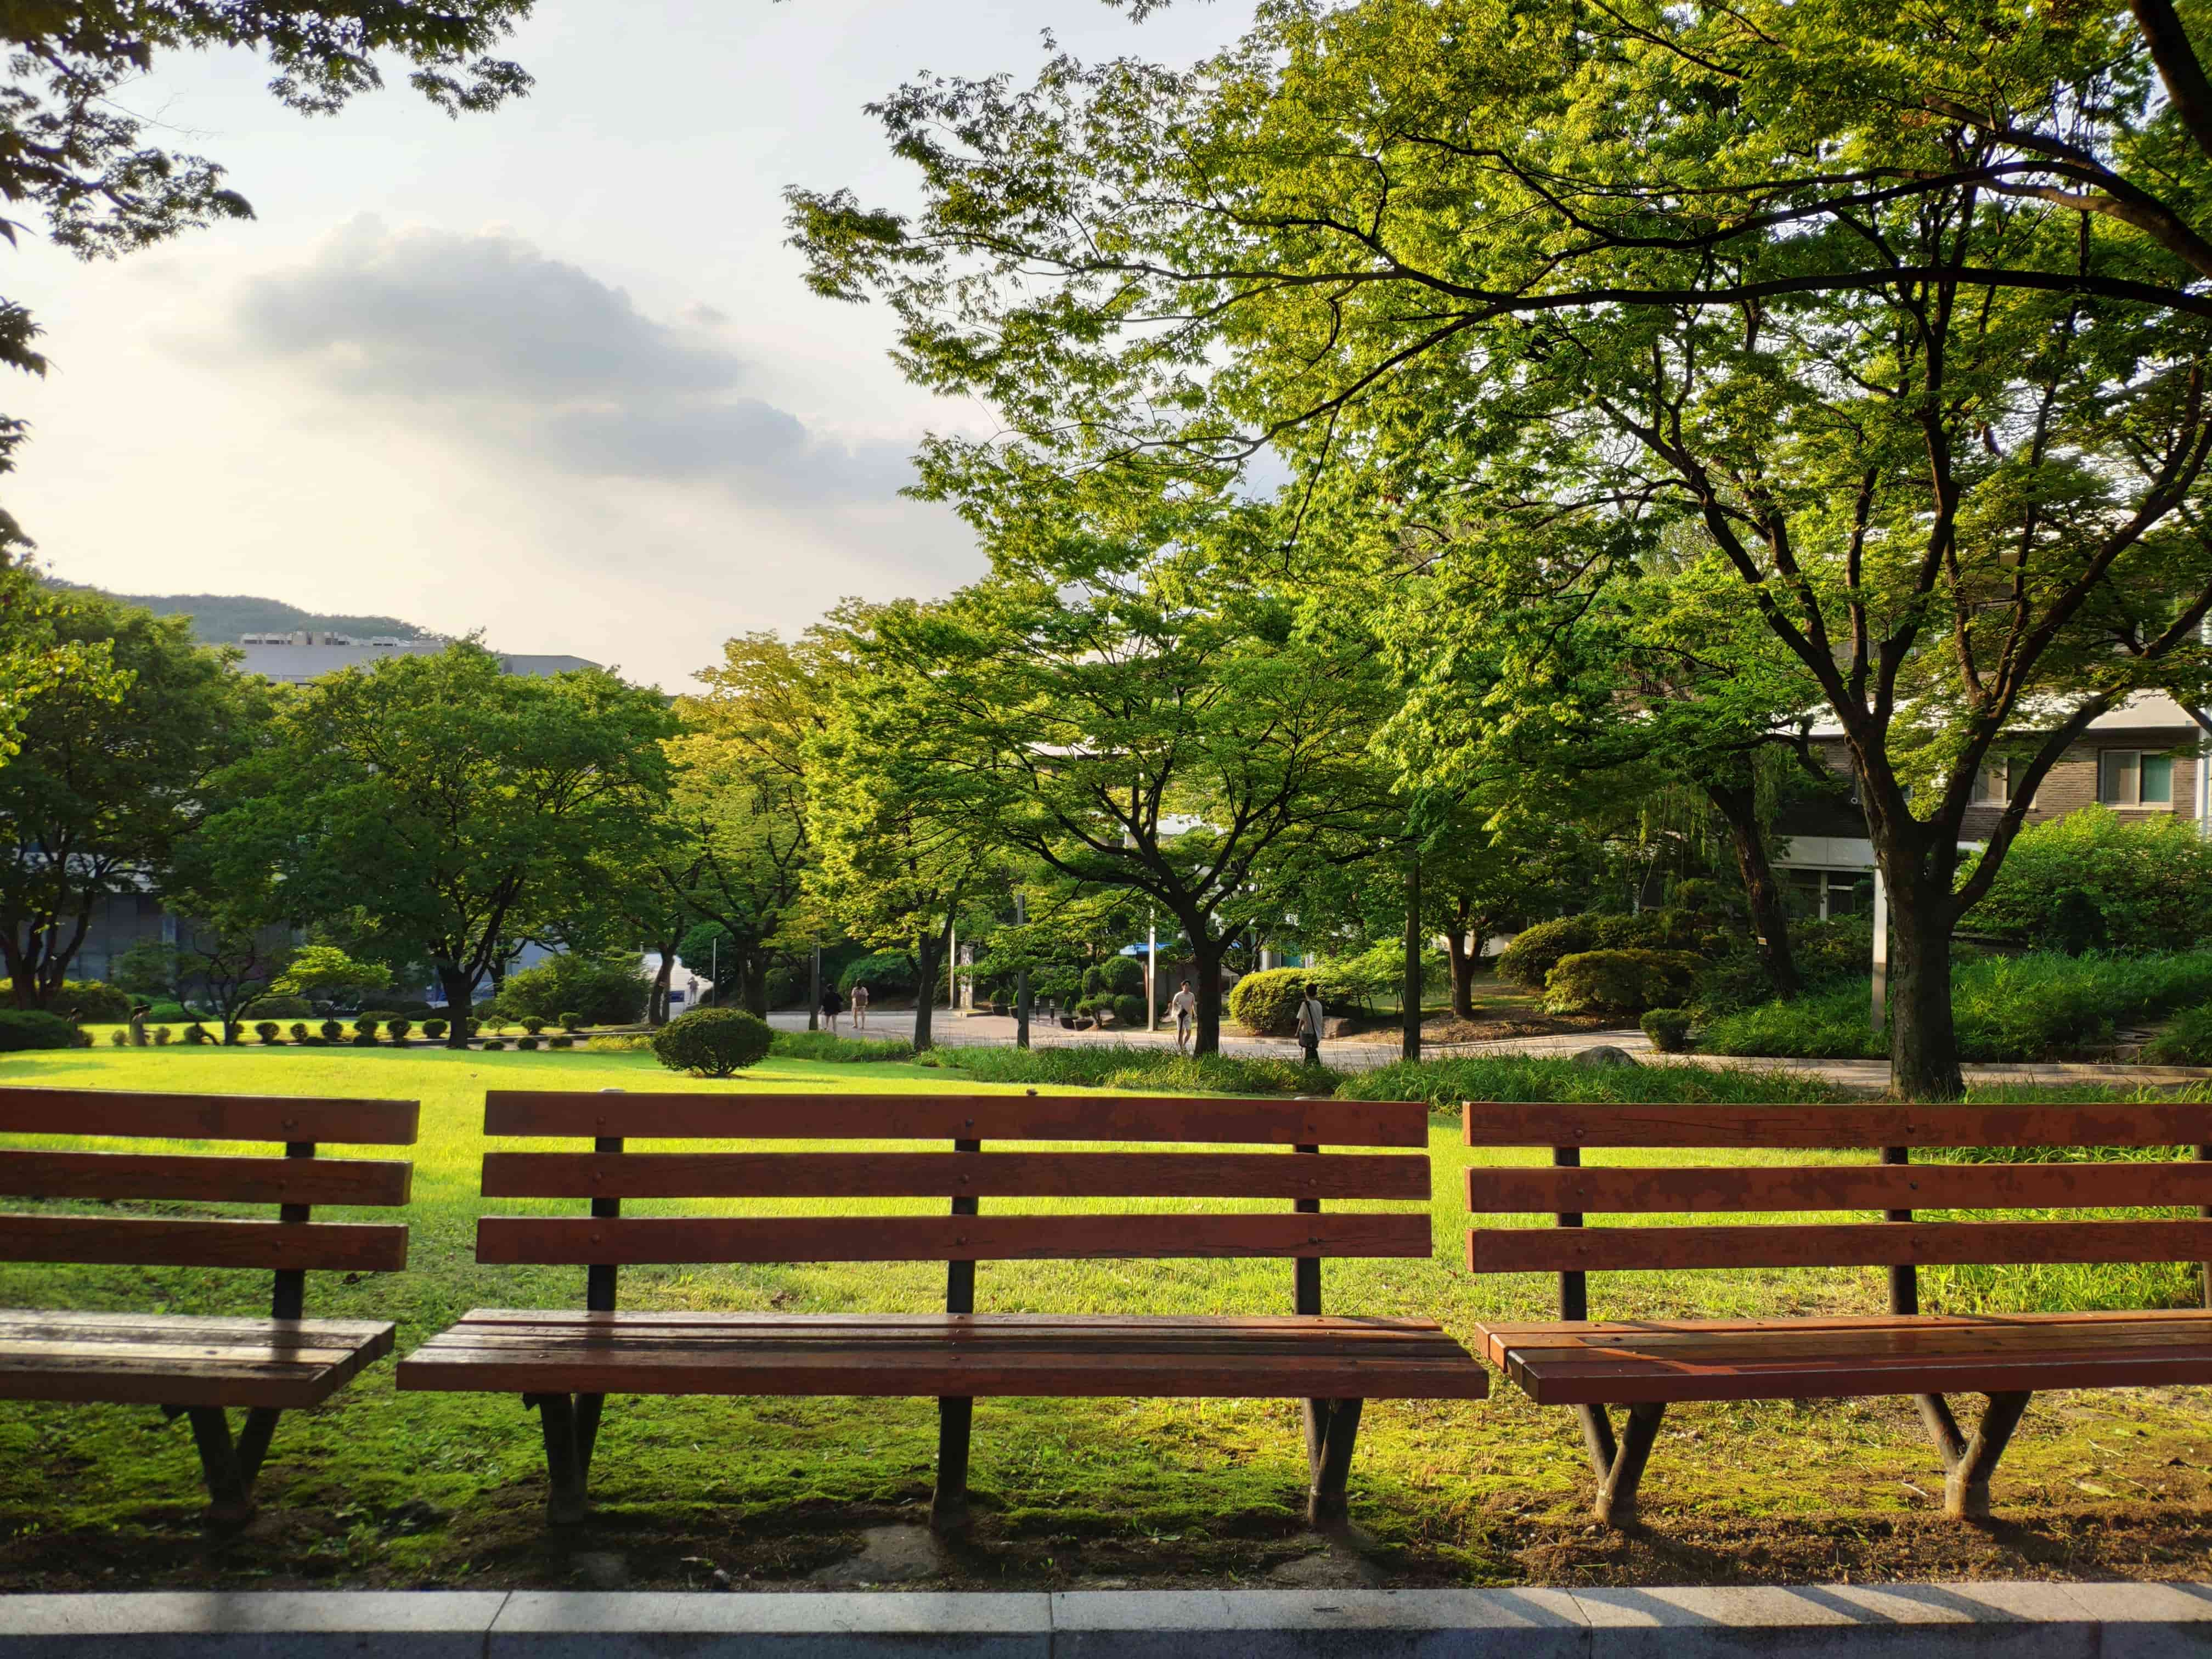
\includegraphics[width=0.9\linewidth]{figures/sightseeing_chair.jpg}
\end{figure}

    
\end{frame}
\plain{May the sun arise from the east.}
\plain{Backup Slides}
\section{BACKUP: Time Integration Method in SU2}

\subsection{Steady Simulations}


\begin{frame}[allowframebreaks]{Implicit Method, Euler Backward Method}

\begin{equation}
\int_{\Omega_{i}} \frac{\partial \boldsymbol{U}_i}{\partial t} d \Omega+\boldsymbol{R}_{i}(\boldsymbol{U}) \approx\left|\Omega_{i}\right| \frac{\mathrm{d} \boldsymbol{U}_{i}}{\mathrm{d} t}+R_{k}(\boldsymbol{U})=0 \quad \rightarrow \quad \frac{\left|\Omega_{i}^{n}\right|}{\Delta t_{i}^{n}} \Delta \boldsymbol{U}_{i}^{n}=-\boldsymbol{R}_{i}\left(\boldsymbol{U}^{n+1}\right)
\end{equation}
where $\Delta \boldsymbol{U}_{i}^{n}=\boldsymbol{U}_{i}^{n+1}-\boldsymbol{U}_{i}^{n}$ means the variables in the cell $i$, $\boldsymbol{R}_i$ is residuals for those variables. However, the residuals at time $n + 1$ are unknown, and linearization about $t^n$ is
needed:

\begin{multline}
    \boldsymbol{R}_{i}\left(\boldsymbol{U}^{n+1}\right)=\boldsymbol{R}_{i}\left(\boldsymbol{U}^{n}\right)+\frac{\partial \boldsymbol{R}_{i}\left(\boldsymbol{U}^{n}\right)}{\partial t} \Delta t_{i}^{n}+\mathcal{O}\left(\Delta t^{2}\right)\\=\boldsymbol{R}_{i}\left(\boldsymbol{U}^{n}\right)+\sum_{j \in \mathcal{N}(i)} \frac{\partial \boldsymbol{R}_{i}\left(\boldsymbol{U}^{n}\right)}{\partial \boldsymbol{U}_{j}} \Delta \boldsymbol{U}_{j}^{n}+\mathcal{O}\left(\Delta t^{2}\right)
\end{multline}

\begin{equation}
\left(\frac{\left|\Omega_{i}\right|}{\Delta t_{i}^{n}} \delta_{i j}+\frac{\partial \boldsymbol{R}_{i}\left(\boldsymbol{U}^{n}\right)}{\partial \boldsymbol{U}_{j}}\right) \cdot \Delta \boldsymbol{U}_{j}^{n}=-\boldsymbol{R}_{i}\left(\boldsymbol{U}^{n}\right),
\end{equation}

If a flux $\tilde{F}_{i j}$ has a stencil of points
${i,j}$, then contributions are made to the Jacobian at four points:
\begin{equation}
\frac{\partial \boldsymbol{R}}{\partial \boldsymbol{U}} :=\frac{\partial \boldsymbol{R}}{\partial \boldsymbol{U}}+\left[\begin{array}{ccccc}{\ddots} & {} & {} & {} & {} \\ {} & {\frac{\partial \tilde{F}_{i j}}{\partial U_{i}}} & {\cdots} & {\frac{\partial \tilde{F}_{i j}}{\partial U_{j}}} \\ {} & {\vdots} & {\ddots} & {\vdots} \\ {} & {-\frac{\partial \tilde{F}_{i j}}{\partial U_{i}}} & {\cdots} & {-\frac{\partial \tilde{F}_{i j}}{\partial U_{j}}} \\ {} & {} & {} & {\ddots}\end{array}\right]
\end{equation}
The position of these four terms are to be checked.


The matrix is very large and contains $(\text{Cell Num} * \text{Variable Num})^2$ components. If one doesn't use the implicit methods in the time-stepping procedure, then there is no necessity to solve the huge sparse linear algebra problem subtly, because all components of the matrix are allocated at the diagonal line.  

Note that, despite implicit schemes being unconditionally stable in theory, a specific value of $\Delta t_i^n$ is needed
to relax the problem. SU2 uses a local-time-stepping technique to accelerate convergence to a steady state.
Local-time-stepping allows each cell in the mesh to advance at a different local time step. Calculation of the
local time step requires the estimation of the eigenvalues and first-order approximations to the Jacobians at
every node i according to

\begin{equation}
\Delta t_{i}=N_{C F L} \min \left(\frac{\left|\Omega_{i}\right|}{\lambda_{i}^{\operatorname{conv}}}, \frac{\left|\Omega_{i}\right|}{\lambda_{i}^{v i s c}}\right)
\end{equation}

where $N_{CFL}$ is the Courant-Friedrichs-Lewy (CFL) number, $\left|\Omega_{i}\right|$ is the volume of the cell $i$ and $\lambda_{i}^{v i s c}$
is the integrated convective spectral radius computed as

\begin{equation}
\lambda_{i}^{c o n v}=\sum_{j \in \mathcal{N}(i)}\left(\left|\vec{u}_{i j} \cdot \vec{n}_{i j}\right|+c_{i j}\right) \Delta S
\end{equation}

where $\vec{u}_{i j}=\left(\vec{u}_{i}+\vec{u}_{j}\right) / 2$, and $c_{i j}=\left(c_{i}+c_{j}\right) / 2$ denote the velocity and the speed of sound at the cell face.
$\vec{n}_{i j}$ denotes the normal direction of the control surface and $\Delta S$, its area. On the other hand, the viscous
spectral radius $\lambda_{i}^{v i s c}$ is computed as
\begin{equation}
\lambda_{i}^{v i s c}=\sum_{j \in \mathcal{N}(i)} C \frac{\mu_{i j}}{\rho_{i j}} S_{i j}^{2}
\end{equation}
where $C$ is a constant, $\mu_{i j}$ is the sum of the laminar and eddy viscosities in a turbulent calculation and $\rho_{i j}$
is the density evaluated at the midpoint of the edge ${i,j}$.

\end{frame}

\begin{frame}[allowframebreaks]{Dual-Time-Stepping}
\begin{equation}
\frac{\partial \boldsymbol{U}}{\partial \tau}+\boldsymbol{R}_{i}^{*}(\boldsymbol{U})=0
\end{equation}
with
\begin{equation}
\begin{aligned} R_{i}^{*}(\boldsymbol{U})=& \frac{3}{2 \Delta t} \boldsymbol{U}_{i} \\+& \frac{1}{\left|\Omega_{i}\right|^{n+1}}\left(\boldsymbol{R}_{i}(\boldsymbol{U})-\frac{2}{\Delta t}\left|\Omega_{i}\right|^{n} \boldsymbol{U}_{i}^{n}+\frac{1}{2 \Delta t}\left|\Omega_{i}\right|^{n-1} \boldsymbol{U}_{i}^{n-1}\right) \end{aligned}
\end{equation}
for second-order accuracy in time (backward difference formula),
where $\Delta t$ is the physical time step, $\tau$ is a fictitious time used to
converge the steady-state problem, $\boldsymbol{R}_i(\boldsymbol{U})$ denotes the residual of the
governing equations.

\end{frame}
\appendix

\begin{frame}[allowframebreaks]
\frametitle{Bibliography}


\nocite{*}
\printbibliography[heading=none]

\end{frame}


\end{document}